\documentclass[11pt,a4paper]{article}

% -------------------------------------------------------
% Page layout and typography
% -------------------------------------------------------
\usepackage[margin=2.5cm]{geometry}
\usepackage[T1]{fontenc}
\usepackage[utf8]{inputenc}
\usepackage{lmodern}
\usepackage{microtype}
\usepackage{setspace}
\onehalfspacing

% -------------------------------------------------------
% Tables, figures and maths
% -------------------------------------------------------
\usepackage{graphicx}
\usepackage{float}
\usepackage{booktabs}
\usepackage{tabularx}
\usepackage{longtable}
\usepackage{array}
\usepackage{amsmath}
\usepackage{siunitx}
\usepackage{gensymb}

% -------------------------------------------------------
% TikZ figures
% -------------------------------------------------------
\usepackage{tikz}
\usetikzlibrary{
    arrows.meta,
    positioning,
    shapes.geometric,
    shapes.misc,
    calc,
    fit,
    backgrounds
}

% -------------------------------------------------------
% References and links
% -------------------------------------------------------
\usepackage[round,authoryear]{natbib}
\usepackage[hidelinks]{hyperref}
\usepackage[nameinlink,noabbrev]{cleveref}

% -------------------------------------------------------
% Metadata
% -------------------------------------------------------
\title{
Wildfire as an Emerging Systemic Mountain Risk in the European Alps:\\
Processes, Modelling Requirements and Cascading Impacts
}

\author{
Author Name$^{1,*}$ \\
\small $^{1}$Affiliation, Department, Institution, City, Country \\
\small $^{*}$Corresponding author: email@domain.org
}

\date{}

% -------------------------------------------------------
% Begin document
% -------------------------------------------------------
\begin{document}

\maketitle


\begin{abstract}
\noindent
Wildfire has been treated as a Mediterranean and lowland problem, and the European Alps have sat at the margin of European fire science. That position is no longer tenable: fire activity in European mountains has migrated upslope by roughly 72\,m per decade since 2000, fire danger is projected to rise across the whole Alpine arc under every emissions pathway, and land abandonment has assembled fuel continuity on steep ground that was open pasture a century ago. Synthesising evidence across climate, fuels, fire behaviour, hazard modelling, silviculture and governance, we argue that Alpine wildfire is not a scaled-down Mediterranean problem but a structurally different one. The fire-size distribution is heavy-tailed, with around 80\% of fires burning under a hectare while the largest tenth account for most burnt area, and fires act on forests whose managed function is to hold rock, snow and sediment above fixed settlement and infrastructure, so consequence is decoupled from area burnt. Consequence follows several pathways: direct loss of protective structure, a geomorphic cascade in which fire lowers the rainfall threshold for erosion, debris flow and rockfall over a window lasting from three years to, at subalpine elevations, effectively permanent, and an ecological loss whose sign differs between closed-forest and open-habitat species and whose faunal term is unmeasured. Because the asset at risk is protective function rather than timber, the response is substantially a forestry problem, and management capacity is a first-order determinant of outcome rather than a residual after climate. We show why the linear prevention instruments of lowland practice transfer awkwardly to terrain where a fuel break is a platform for ground suppression that crews cannot reach, and why an apparatus producing hazard surfaces without exposure or vulnerability terms cannot yet produce Alpine risk. A research agenda follows from what the observational record can support.
\end{abstract}

\noindent\textbf{Keywords:}
wildfire; European Alps; mountain risk; fire regime change; post-fire geomorphic cascade; protection forest; silviculture and fuel management; drought and water availability; wildfire economics; multi-hazard risk assessment


% =======================================================
\section{Introduction}
\label{sec:intro}
% =======================================================

\subsection{An emerging fire frontier in temperate mountains}

The geography of European fire science has followed the geography of burnt area. Because the Mediterranean basin accounts for most of the continent's burning, it has also supplied most of the continent's fire statistics, operational danger rating and prevention doctrine. Two developments are now unsettling that arrangement. The first is that the continental distribution of fire activity is shifting: burnt area has been declining in the Mediterranean while increasing in mid- and high-latitude regions where fuel is abundant and where plant communities carry little adaptation to fire \citep{miller_compounding_2025}. The second is that the shift has a vertical component. Across eight European mountain regions between 2000 and 2025, the median elevation of fires larger than 30\,ha rose from 910 to 1004\,m, the ninetieth percentile from 1353 to 1460\,m, and the ten largest annual fires from 1451 to 1777\,m, an upslope migration of approximately 72\,m per decade driven principally by vapour pressure deficit \citep{beloiu_climatedriven_2026}.

The pattern is not confined to mountains. In the Netherlands, a densely populated temperate country with no fire tradition, 3{,}667 landscape fires were recorded between 2017 and 2022, averaging 611 a year and around 405\,ha annually, with a mean fire size of 1.5\,ha and 88\% of events burning less than a hectare, concentrated in spring and in summer drought and almost entirely human-ignited \citep{stoof_temperate_2024}. That profile is close to the Alpine one, and so is the institutional position it describes: fire services specialised in urban firefighting, and neighbouring countries without systematic wildfire statistics at all.

The European context in which that projection sits has since moved. European burnt area and fire carbon emissions reached record levels in 2025, concentrated in the Iberian Peninsula, and the same assessment finds that emissions mitigation has already reduced projected end-of-century burnt area in extreme events, by 4\% to 23\% under a high pathway relative to the worst-case scenario now considered implausible, and by a further 5\% to 36\% under a Paris-consistent pathway \citep{burton_state_2026}. The trajectory of Alpine fire danger is therefore conditional on mitigation as well as on adaptation, which is not how it is usually presented.

How much of that increase is realised is not, however, fixed by climate alone. Coupling two fire models to a dynamic global vegetation model across Europe, intensified fire weather alone is projected to raise annual burned area by around 39\% under SSP1-2.6 and by nearly 192\% under SSP3-7.0 by the end of the century, but continued improvement in fire management capacity would reduce burned area by 72\% to 92\% relative to scenarios without such improvement, while still leaving net increases in roughly 55\% of Europe's fire-prone regions, with the hotspots of increase under the higher pathway concentrated in foothills and medium-elevation terrain including the Alps, Pyrenees, Carpathians and Massif Central \citep{billing_future_2026}. Management capacity is therefore a first-order determinant of Alpine outcomes, not a residual after the climate signal has been counted.

Fire is therefore arriving in terrain where neither the science, the management apparatus, nor the exposed population has accumulated experience of it. The deficit was named more than a decade ago from inside Alpine forestry: reviewing the risks facing Alpine Space forests, the MANFRED consortium observed that the history of active fire suppression meant fire risk did not receive full attention in the Alps, while noting that future climate conditions might well require an improved alerting system to prevent devastating forest fires \citep{jandl_management_2013}. The intervening decade has supplied the climate signal; the attention has followed more slowly. The scale of the projected change is large relative to that baseline. Across the Alps, hazard probability is projected to increase by 15.5\% under SSP1-2.6 and by 35.4\% under SSP5-8.5, with the largest relative increases in the northern and eastern sectors rather than in the already fire-affected south-west \citep{gerberding_mapping_2025}. In adjacent central European landscapes, a regional large ensemble under RCP8.5 places the emergence of the forced fire-danger signal before 2050 in every subregion examined, and shifts present-day hundred-year fire weather to a ten-year recurrence by 2090 \citep{miller_climate_2024}. Both results describe a hazard moving from the anecdotal to the routine within the planning horizon of the institutions that would have to absorb it.

\subsection{Why mountain fire is a distinct problem}

Three features of mountain terrain prevent the Mediterranean toolkit from transferring cleanly.

Terrain reorganises the atmosphere. The assumption of a continuous fire-weather field, interpolable from valley-floor stations, loses validity where upper winds interact with complex relief to produce discontinuous and locally amplified surface conditions \citep{sharples_overview_2009}. The magnitude of this effect has been quantified: atmospheric profiles capable of generating enhanced surface winds occurred in 6.5\% of cases over the least rugged terrain of a Tasmanian study domain but in 40.2\% over the most rugged, and fire simulations driven by surface winds alone degraded systematically as terrain complexity increased \citep{ozaki_impact_2022}.

Terrain reorganises fire behaviour. Rate of spread accelerates non-linearly with upslope angle, roughly two and a half times between 20\degree{} and 30\degree{} in controlled experiments, with the dominant preheating mechanism switching from radiation to convection across that range and flame attachment appearing near 25--30\degree{} in confined geometries \citep{hayajneh_wind_2026}. The landscape-scale consequence is measurable: across 21 Swiss pyroregions, the length of upslope paths within forested area combined with the aggregation of that area explains between 56\% and 65\% of the variance in large-fire statistics, without any weather term \citep{conedera_linking_2024}.

Most importantly, in mountains the fire is rarely the end of the event. Alpine forests are managed substantially for their protective function against rockfall, avalanche and shallow landslide, and fire removes that function over a window measured in years \citep{melzner_wildfire-induced_2025, melzner_brief_2019}. The asset at risk is typically not the stand that burns but the settlement, road or railway beneath it.

\subsection{Objective and argument}

The Alpine fire community already has a consensus statement. The EUSALP white paper of February 2020 set out the state of knowledge for policy makers, established the arc-wide statistical baseline, identified the loss of protective function as the central concern, and proposed a costed integrated fire management framework \citep{muller_forest_2020}. This review takes that position as its point of departure and asks what the evidence has since established. In several places that evidence complicates the 2020 position rather than confirming it, and where it does we identify the finding responsible.

This review assembles the evidence needed to treat Alpine wildfire as a systemic mountain risk rather than as a forest-loss problem. Its argument has four parts, two of which extend the 2020 position and two of which complicate it.

The two that extend it begin from framings already established there. The Alpine fire regime is structurally distinct rather than merely smaller than the regimes on which European fire science was built; that claim was advanced in 2020 from the arc-wide statistics, and subsequent work has made it quantitative in the vertical dimension, through a measured upslope migration of fire activity in European mountains \citep{beloiu_climatedriven_2026}, and in the operational one, through terrain-conditioned estimates of the difficulty of containment \citep{cardil_assessing_2025}. Because what fire destroys in the Alps is a managed protective function, the response is substantially a forestry problem; that identification is also inherited, but the material for acting on it is not, and we treat silviculture, fuel treatment and post-fire restoration as first-order subjects on the strength of monetised valuations of the protective service \citep{accastello_asforesee_2019, moos_climate_2021}, a controlled Alpine prescribed-burning trial \citep{gamba_prescribed_2025} and severity-resolved measurement of the interval over which protection is lost \citep{melzner_wildfire-induced_2025}.

The two that complicate it are the substance of the review. Consequence in the Alps is decoupled from burnt area and runs through several pathways at once (direct loss of protective structure, ecological and hydrological change, and a geomorphic cascade in which fire sets a susceptibility that a later hydro-meteorological event realises), so that the geomorphic pathway, although the least represented in current assessment, should be understood as one term in the loss function rather than as the whole of it. Part of that pathway also falls outside the return-period logic in which mountain hazard is conventionally expressed, since a burnt Alpine catchment has been observed to respond to a rainfall intensity below the threshold that unburnt basins of its type require \citep{laporta_postwildfire_2025}. And the current apparatus omits processes that add to hazard while stopping short of risk, since the exposure and vulnerability terms that would convert a burn probability into an expected loss exist as instruments but have not been assembled for the arc; the Alpine data record is meanwhile too thin to justify the conventional remedy of added complexity, and we use that constraint, rather than any appeal to greater model sophistication, to organise a research agenda.

A further consideration motivates the exercise. The 2020 statement is a policy white paper rather than a contribution to the scientific record, so its evidence base is not indexed, peer reviewed or available for citation and appraisal in the ordinary way, and its positions cannot be tested or extended by the community that would have to act on them. Setting that position against the peer-reviewed literature that has since accumulated, and stating for each element how securely it is now supported, is itself part of what a review can supply.


% =======================================================
\section{Review Design and Scope}
\label{sec:scope}
% =======================================================

\subsection{Scope and inclusion rule}

The geographical core is the Alpine arc as delimited by the Alpine Convention, covering Austria, France, Germany, Italy, Liechtenstein, Monaco, Slovenia and Switzerland. This is the perimeter within which harmonised Alpine fire statistics were first assembled \citep{valese_wildfires_2011, muller_forest_2020}, within which arc-scale hazard mapping has been performed \citep{gerberding_mapping_2025}, and across which the practitioner community is organised \citep{hoang_stakeholders_2026}.

We depart from that perimeter under two controlled conditions. Evidence from other European mountain systems (Pyrenees, Carpathians, Apennines, Dinarides, Tatras) is admitted where it addresses a process for which Alpine evidence is absent rather than merely thin. Evidence from non-European mountain systems is admitted where the process is physically general and the Alpine literature is silent. Terrain reorganises atmospheric flow and thereby fire weather, slope and wind interact non-linearly to set spread rate, fire removes the vegetation and soil structure that hold sediment on steep ground, and terrain conditions the feasibility of suppression: each of these is a physical relationship established outside Europe and applicable within it \citep{sharples_overview_2009, hayajneh_wind_2026, santi_wildfire_2022, morell_sediment_2021, cardil_assessing_2025}. Imported material establishes that a process exists and characterises its mechanism; it is never used to quantify Alpine magnitude.

\subsection{Identification, screening and evidence weighting}

The corpus was assembled by bidirectional citation snowballing from a seed set rather than by systematic database querying, and we state this plainly because the distinction matters for how the review should be read. Backward chaining extracted and de-duplicated the reference lists of the seed publications; forward chaining retrieved citing works through open citation infrastructure; a subsequent expansion phase added open-access publications whose full text could be retrieved and archived. Screening applied a graded inclusion rule (fire and the Alps; fire and another mountain system as comparative evidence; Alpine process without fire, or European fire without mountains, as context; generic fire science excluded), with every decision and its reason recorded. Counts at each stage, and the reasons for exclusion, are reported in Appendix~\ref{app:protocol}, which documents the protocol as executed. The synthesis is structured and narrative: it applies an explicit and reproducible identification and screening procedure, and reports the resulting evidence thematically.

The synthesis is thematic rather than meta-analytic, and this follows from the evidence rather than from preference. Alpine fire studies differ in their definitions of severity, in burnt-area thresholds, in reporting periods and in the administrative basis of their fire records, so effect sizes are not commensurable across studies; the same obstacle has been documented for the neighbouring literature on land abandonment and disturbance, where study sites cluster strongly and coverage across disturbance types is uneven \citep{mantero_influence_2020}.

Because much of the Alpine evidence base consists of individual documented events, we adopt an explicit convention for weighting it. Case evidence is used to establish that a process operates, to characterise its mechanism and to bound its magnitude in one setting; it is not used to estimate a regional parameter, and we state the number of independent cases wherever a claim rests on fewer than three. Where a mechanism is established outside Europe, it is identified as imported and used for mechanism only. Where a claim is supported by multiple independent Alpine studies, that is said. Readers should treat single-case magnitudes as existence proofs with an observed value attached, not as central estimates, and several of the quantities cited in Sections~\ref{sec:cascade} and~\ref{sec:silviculture} fall into this category.


% =======================================================
\section{The Alpine Fire System}
\label{sec:system}

\subsection{Regime structure: fire size, seasonality and ignition}

The Alpine fire regime is defined less by its magnitude than by its shape. Harmonised statistics for 2006--2017 place annual fire numbers between 37 in Slovenia and 1043 in Italy, and annual burnt area between 64\,ha in Austria and 9984\,ha in Italy; normalised by forest area, the range spans two orders of magnitude, from 0.22 to 44.13\,ha burnt per 10{,}000\,ha of forest per year \citep{muller_forest_2020}. Roughly 80\% of Alpine fires burn less than one hectare, and median fire size falls below 0.1\,ha in Austria, Germany and Switzerland. The distribution is nonetheless strongly heavy-tailed: in the French and Italian Alps the mean fire covers about a hectare, yet the 10\% of fires exceeding ten hectares account for some 85\% of total burnt area \citep{muller_forest_2020}. Both halves of that statistic matter, and citing either alone misleads. The many small fires define what monitoring must detect and what suppression routinely handles; the few large ones define the burnt area, and, in an Alpine setting, the events capable of removing protective function across a whole slope. For comparison, the mean patch size of all detected forest disturbance across Europe over three decades is 1.09\,ha \citep{senf_mapping_2021}, so Alpine fire sits at the fine end of an already fine-grained disturbance regime.

Seasonality is bimodal, and this is the regime's most consequential structural feature. A spring season of fast-spreading surface fires at low elevation peaks in March and April; a summer season peaks in July and August; and winter fires occur in foehn-influenced valleys \citep{valese_wildfires_2011, muller_forest_2020}. The pattern is not confined to the Alpine arc: in the Czech Republic the same bimodality appears with an April peak and a July--August peak, the former attributed to forestry operations resuming after winter and the latter to heat, drought and tourism, with a threshold response above 18\,\degree C \citep{bercak_combination_2024}. The two modes have different controls, and there is no reason to expect them to change in step.

Ignition is mixed in a way that has no Mediterranean analogue. Human causes account for approximately 90\% of Alpine fires, but lightning contributes around 10\% regionally and up to half of summer ignitions in some areas, concentrated on southern slopes and at higher elevation \citep{muller_forest_2020, valese_wildfires_2011}. That lightning frequency emerges as one of the three strongest predictors of fire hazard in Alpine-scale statistical mapping, alongside mean annual temperature and precipitation seasonality \citep{gerberding_mapping_2025}, is diagnostic: no Mediterranean hazard model would rank it so highly. Anthropogenic ignition follows the access network rather than population alone: railway, forest-road and hiking-trail density, together with agricultural and forestry activity, are the operative predictors at national scale in Austria, and they resolve to municipality-level danger classes usable for prevention targeting \citep{arndt_modeling_2013}.

The two modes are separable statistically as well as descriptively, and they are driven by different variables. In an inner-Alpine valley, summer ignition responds to maximum temperature and to precipitation of the wettest month, winter forest fire to precipitation and elevation, and proximity to infrastructure matters in winter but not in summer; negligence in agro-silvicultural activity accounts for around two-thirds of identified ignitions, and the lightning share rose over the study period \citep{vacchiano_modeling_2018}. A single annual model fitted to this system would average across processes with different drivers acting in different seasons.

The regime also regionalises coherently. Three clusters (Southern, Northern and Maritime Alps) separate the high fire density of the southern slope from the substantially lower burnt-area fraction of the north, and are distinguished by drought frequency and duration, vegetation type, mean elevation, valley orientation, population density and educational level \citep{conedera_characterizing_2018}. With only ten years of record the classification functions as a baseline against which future regime shifts and anomalous seasons can be detected rather than as a description of a stable state, and on present evidence fire does not rival storms and bark beetles for damage in the Alpine region, although future regimes may evolve under climatic and socio-economic change \citep{conedera_characterizing_2018}. That is a more measured framing than much of the recent literature adopts, and this review adopts it.

\subsection{Climatic controls and their relaxation}

The controlling gradients are elevation, the divide between the moist northern and insubric southern slopes, and the contrast between dry continental inner valleys and wetter outer ranges. Elevation currently supplies the hard constraint, through snow cover and through temperature-limited fuel drying, and it is precisely this constraint that warming is relaxing. Mountain warming is elevation-dependent, with the snow- and ice-albedo feedback among the principal mechanisms, in an amplification analogous to that of the Arctic \citep{rangwala_climate_2012}; and reduced snow-cover duration is already reshaping the seasonal economy of high-altitude Alpine municipalities \citep{pede_mountain_2022}.

The proximate mechanism linking climate to fire is fuel moisture rather than temperature. Across European climate regions, multi-month drought indices, soil moisture deficit and vapour pressure deficit are the strongest and most consistent drivers of fire activity, and their interactions are region- and season-specific: productivity deficits matter in southern Europe in summer, whereas in northern Europe summer preconditions combine moisture deficit with productivity \emph{surpluses}, so that fuel production and fuel drying compound rather than trade off \citep{miller_compounding_2025}. The same variable dominates the ignition side. In a five-site European ignition model, the annual anomaly in dead fine fuel moisture content ranked as the most influential predictor at every site \citep{gelabert_assessing_2025}, and vapour pressure deficit is likewise the strongest predictor of burnt area in the mountain upslope analysis \citep{beloiu_climatedriven_2026}.

Two structurally different droughts drive extreme European fire, and the distinction matters for the Alps because the two Alpine seasons plausibly respond to different ones. Analysis of extreme events in south-eastern France separates a press drought, in which a long-lasting water deficit produced by reduced precipitation and elevated evapotranspiration intensifies wind-driven fires, from a hot drought in which a comparable deficit combines with a summer heatwave to intensify heat-induced fires \citep{ruffault_extreme_2018}. Alpine spring fires, carried by cured herbaceous fuel under foehn, correspond mechanistically to the first; the emerging high-elevation summer fires, associated with extreme atmospheric aridity above 1400\,m \citep{beloiu_climatedriven_2026}, correspond to the second. A danger system calibrated on one will not represent the other, and an Alpine climate projection that reports a single aggregate trend conceals which of the two is changing.

The Alpine-specific trend evidence comes from 25 long-term stations distributed across six Alpine countries and grouped into climatically homogeneous regions. Mean annual fire danger, taken as the median of seven danger indices, rose clearly and significantly south and west of the Alps, while north of the Alps and in the inner Alpine valleys a high proportion of trends were not statistically significant; at the 95th percentile, however, almost every station showed a trend towards higher index values \citep{wastl_recent_2012}. Warming is therefore lifting the extreme tail of Alpine fire danger even where the mean is not moving detectably, which is the pattern most likely to be missed by monitoring designed around averages.

The distinction between fire danger and realised fire regime should be kept sharp, because the Alps have much evidence for the first and little for the second. European fire danger showed no clear trend between 1960 and 1999 but a significant increase in southern and eastern Europe from 1980 onward, with correlations between fire-season weather indices and burnt area of order 0.6 \citep{venalainen_temporal_2014}. Detecting a corresponding regime change in the Alps is harder: records are short and administratively fragmented, fires are small enough that recording thresholds dominate the statistics, and the strong seasonal and topographic structure allows compensating changes to cancel in regional aggregates. Under these conditions the absence of a signal is weak evidence of its absence.

One consequence for anticipation deserves noting. A global analysis of thirteen climate teleconnections found that collectively they modulate around half of global burnt area, but that these relationships are markedly weaker in Europe than on other continents, with only the North Atlantic Oscillation and the East Atlantic pattern showing consistent associations in temperate regions \citep{cardil_climate_2023}. Seasonal fire forecasting from remote climate modes will therefore deliver less in the Alps than in regions where a single mode dominates, which places correspondingly more weight on land-surface and fuel-state monitoring.

Where regrowth happens is economically determined and locally variable. A spatially explicit analysis of the Swiss mountains found forest re-growth concentrated where cultivation costs were high and yield potential low, with non-linear relationships to slope steepness and soil stoniness, and concluded that general policy measures applied across the whole mountain area are unsuitable for preventing abandonment and re-growth, which instead require attention to local characteristics \citep{gellrich_agricultural_2007}. Swiss forest area has risen by roughly a third over the last 150 years, most of it by natural re-growth rather than planting. Fuel accumulation in the Alps is therefore the spatial signature of agricultural marginality, which is also why it concentrates on the steep ground where fire runs longest.

The long view from the driest Alpine valleys supports this reading. Reconstruction of the fire history of Valais, a dry continental valley of the Swiss Alps, treats the fire regime as jointly determined by climatic, vegetation and anthropogenic factors and traces regime shifts across the twentieth century in both Valais and Ticino \citep{zumbrunnen_reconstructing_2010}. Alpine fire regimes have shifted before, under human rather than climatic forcing, which is a caution against attributing any contemporary shift to climate by default.

\subsection{Fuel accumulation, connectivity and disturbance interactions}

The landscape now burning is a recent artefact. Centuries of grazing, litter collection and fuelwood extraction held Alpine forests open in a mosaic that limited spread irrespective of weather; the retreat of that regime has reassembled the fuel bed \citep{bebi_changes_2017}. Expansion is not uniform. It is fastest where recent agricultural abandonment coincides with climatically favourable conditions for establishment, so that anticipating future fuel continuity requires knowing how the timing of land-use change intersects with growth conditions, not simply where abandonment occurred \citep{garbarino_contrasting_2020}. The generalisation that abandonment monotonically increases fire hazard should nonetheless be treated as a regionally supported finding rather than a law, since for disturbances other than fire the reported effects of abandonment are inconsistent and sometimes opposite in sign \citep{mantero_influence_2020}.

Quantifying the vertical component, and for one intensively surveyed Central Swiss valley, the treeline advanced by an average of 10\,m per decade between the early 1970s and 2012, with local maxima of 42\,m per decade; decisively, only 21\% of new trees represented advance beyond the former treeline while 79\% were infilling below it \citep{frei_evidence_2023}. Fuel is therefore not merely climbing but densifying, and densification below the treeline is what converts scattered stands into continuous fuel. At Alpine scale, 24\% of the 10.5 million hectares of forest is in an open-canopy structural state, concentrated at high elevations, forest edges and warm dry sites \citep{stritih_alternative_2023}, the same positions where fuel is now filling in.

The behavioural consequence follows directly. Where fuel connectivity and slope length jointly govern large-fire likelihood \citep{conedera_linking_2024}, expansion onto steep marginal ground that was abandoned first increases exactly the quantity that matters. This is the mechanism by which a landscape can become more fire-prone without any change in weather.

That regime now has a measured European baseline resolved by causal agent. Classification of more than 3.8 million fire, wind and bark beetle events across European forests between 1985 and 2023 separates fire regimes on a north--south gradient, severe and rare in boreal and temperate forest against moderate, large and frequent in Mediterranean and transitional forest, and separates wind and beetle disturbance into four regimes of which the frequent and small predominates in Central Europe \citep{miguel_unravelling_2026}. The result that bears hardest on Alpine assessment is not the classification but its instability: about 15\% of grid cells changed regime within the record, fire frequency and severity fell in temperate and Mediterranean forest between the first and second period, and wind and beetle disturbance then rose in severity in temperate forest between the second and third. A disturbance regime is not a fixed property of a region on which a fuel model can be built once.

Fire in the Alps arrives into a disturbance regime, not a quiescent forest, and the interactions are structured rather than additive. Wind, snow break, bark beetle and avalanche shape Alpine stands continuously \citep{bebi_changes_2017}, and at Alpine scale a quarter of forest area is already in an open-canopy structural state, with disturbance initiating transitions to that state in roughly half of cases and recovery to closed canopy taking around 35 years in most forest types \citep{stritih_alternative_2023}.

Disturbance susceptibility is also partly a management artefact rather than a purely climatic one. The MANFRED programme, a transnational Alpine Space collaboration spanning fifteen partners in six countries, concluded that recorded storm damage in Alpine forests is not driven by climate alone, and that the prevailing silvicultural practice of allowing increasingly dense forests to mature has itself produced stand types that are markedly vulnerable to storms \citep{jandl_management_2013}. The fuel and the fragility have a common origin in how the forest has been managed.

What distinguishes fire from the other agents is what it leaves behind. Windthrow appears to leave biological legacies that continue to perform the protective function of the standing forest. In the one Alpine stand where this has been simulated explicitly, rockfall modelling over a windthrown site in the Dolomites found the barrier effect index improved after the storm, with the fallen stand more protective than the forest that preceded it, because lying logs and stumps act as physical obstacles rather than as energy absorbers, and this legacy can persist for up to thirty years until decay and soil contact degrade it \citep{costa_biological_2021}. Fire does not leave that legacy. It consumes fine material, weakens standing stems that subsequently fall without forming an effective barrier, and destroys the litter layer that arrests small blocks \citep{asteriou_assessing_2025}. Two disturbances that produce similar canopy loss therefore produce opposite short-term consequences for slope protection, which is a strong argument against treating fire as one interchangeable member of the Alpine disturbance suite.

The corollary is that salvage decisions after fire cannot simply import the consensus developed after windthrow. Where that consensus advises against salvage in order to retain protective legacies \citep{costa_biological_2021}, the evidence base is itself less categorical than often assumed: eighteen years after a Tatra windstorm, salvaged areas retained an eighth of the deadwood volume of unsalvaged areas but supported higher regeneration diversity, 5.40 against 3.85 species per plot, with unsalvaged plots dominated by Norway spruce \citep{seben_impact_2024}. The trade-off between protective legacy, regeneration composition and future fuel is real, differs between disturbance types, and has not been evaluated for Alpine post-fire sites.

A comparative case marks the boundary of the Alpine trajectory. In the southern Appalachian Mountains decades of suppression preceded a regional outbreak of more than a dozen large wildfires during one of the warmest and driest droughts of the last century, in a landscape whose historical mosaic had been maintained by frequent low- and mixed-severity fire and whose composition had already been reorganised by land-use change \citep{reilly_drivers_2022}. The Alps never had a frequent-fire regime to suppress, so the trajectory is not the same one; what the comparison establishes is only that a landscape whose fuel structure has ceased to match its disturbance history can support a regional outbreak once drought supplies the trigger.

\subsection{Species vulnerability, drought stress and the loading of the fuel bed}

Alpine tree species differ sharply in their capacity to survive fire, and the composition of Alpine forests is being reorganised on a timescale comparable to that of regime change. Simulation of Swiss Alpine landscapes indicates that climate-driven vegetation shifts will exert a larger influence on biomass and species distribution than management, with fire emerging as a property of the simulated landscape that then feeds back on vegetation \citep{schumacher_relative_2006}.

Vulnerability is trait-mediated and now has independent experimental support. Simulation across 4438 French Alpine forest plots showed cold-season fires, about half of all fires there, having limited impact except on low-elevation southern stands, average summer conditions producing highest mortality in mixed and broadleaved low-elevation forests with up to 75\% mortality in coppice, and extremely dry summers producing high mortality across all communities, with the lowest mortality in thick-barked, high-canopied larch stands of the inner Alps \citep{dupire_vulnerability_2019}. Controlled heating of stem discs from six Central European species reproduces that ranking from first principles: bark thickness is the most robust predictor of the time taken for the cambium to reach the lethal threshold, placing larch, Douglas-fir and Scots pine above silver fir and Norway spruce, with beech lowest, and thermal resistance declining with bark moisture and with height on the stem \citep{mutterer_bark_2026}. Two very different methods converge, which is a stronger basis than either alone.

Composition is also a fire outcome, not only a fire input. After a stand-replacing fire in the Rhone valley, recruitment favoured pioneer birch, aspen and willow over the pre-fire larch, spruce and Scots pine, and seedling density tracked moisture availability rather than fire intensity, leading to the conclusion that drought is the limiting factor for post-fire recruitment in the Central Alps \citep{moser_potential_2010}. Palaeoecological records extend the same logic across millennia, with fire and grazing rather than temperature alone determining whether the timberline attains its climatic potential \citep{colombaroli_species_2010}, and with regionally distinct Holocene fire--vegetation trajectories reconstructed for the Dinaric ranges \citep{cagliero_effect_nodate}.

Drought acts on Alpine forests through a chain that is separable into three links, and the fire literature has generally attended to the first while the forest health literature has attended to the second and third.

The first link is fuel moisture, and it is the one already established, though not the one best modelled. A global evaluation across 1{,}603 measurements from 153 experiments in 21 countries found vapour-pressure-deficit models performing competitively over the full moisture range, with mean absolute errors near 4\% and coefficients of determination around 0.4, and machine-learning alternatives improving on them only marginally; below 10\% moisture, however, every approach degraded to a coefficient of determination of about 0.11, which is precisely the range in which spread responds exponentially to dryness \citep{rodrigues_vpdbased_2024}. Fuel moisture is predicted worst where it matters most. Within that limitation, dead fine fuel moisture anomaly is the strongest single predictor of ignition likelihood across European pilot regions \citep{gelabert_assessing_2025}, and multi-month drought indices together with vapour pressure deficit dominate burnt area \citep{miller_compounding_2025, beloiu_climatedriven_2026}.

The second link is physiological, and it converts drought into standing dead fuel. In Scots pine at the dry margins of its range, which includes the inner Alpine valleys, drought-induced mortality proceeds through carbon starvation, as reduced assimilation under water stress depletes the reserves that also fund defence, leaving trees susceptible to pest and pathogen attack \citep{giuggiola_droughtinduced_2010}. Experimental work isolates the interaction: in Norway spruce, simultaneous drought and root-rot infection create competing demands on carbon, since compartmentalising the pathogen and maintaining turgor draw on the same pool, while the infection itself reduces functional sapwood and so compounds water stress; needle starch concentration predicted which saplings died \citep{gomezgallego_interaction_2022}. Scots pine showed no such interaction in the same experiment, which matters because the two species occupy different Alpine positions and would therefore be expected to fail by different routes.

Whether such decline proceeds gradually or abruptly is not settled, and the comparative evidence favours abruptness. In central Chile, more than 90\% of a Mediterranean-type forest browned within fewer than a hundred days under conditions unprecedented across all five Mediterranean-type ecosystems, with long-term recovery uncertain given a continuing decline in regional water balance \citep{miranda_widespread_2023}. The setting is not Alpine and the magnitude does not transfer, but the mode does: drought-driven decline can be synchronous and regional rather than incremental, which is the behaviour that would convert a gradual fuel-loading trend into a step change.

The third link is that dead and weakened trees are fuel. This is asserted in the Alpine hazard literature but not represented in its models: projections of Alpine fire hazard note that drought, heatwaves and storms favour bark beetle outbreak and windthrow and thereby increase the availability of flammable material, while conceding that the pathway is absent from the projection \citep{gerberding_mapping_2025}. Since disturbance is constitutive of Alpine forest dynamics rather than exceptional \citep{bebi_changes_2017}, and since European forest disturbance frequency has been increasing over three decades while severity has been falling \citep{senf_mapping_2021}, this omission is unlikely to be small.

The chain closes on itself in a way that has consequences for management. The chain therefore closes on a single silvicultural lever: in inner Alpine valleys, intervention against drought stress and intervention against fuel are substantially the same operation, an alignment developed in Section~\ref{sec:silviculture} and one that management planning does not currently exploit.

\subsection{Mountain meteorology and terrain-driven fire behaviour}

Synoptic control on Alpine fire danger has been characterised directly. Combining a sixty-year weather-type classification with station data, danger indices and observed fires across the Alps, elevated danger occurred predominantly under persistent anticyclonic situations or in the lee of the range under katabatic foehn, with the southern Alpine region the most fire-prone; differences between weather types narrowed for indices representing deeper soil layers, reflecting longer drying response times \citep{wastl_largescale_2013}. Foehn is therefore not an incidental local phenomenon but one of the two synoptic configurations that generate Alpine fire danger.

Alpine wind systems are the mechanism converting small ignitions into fast fires, and they operate in three families: foehn, which can strip tens of percentage points of relative humidity within hours and is associated with the late-winter and spring fires of inner and southern valleys; thermally driven diurnal circulations, whose anabatic day and katabatic night reversal imposes a spread-direction cycle with no lowland analogue; and terrain channelling of the synoptic flow along valley axes and through cols. Steep Alpine topography exerts a controlling influence on all three, and thereby on fire type, intensity and burn severity \citep{melzner_wildfire-induced_2025}.

The observational evidence for terrain-driven behavioural anomaly in the Alps rests, at present, on a single documented case. During the 2018 Hallstatt fire in Austria, vertical rock walls, anabatic winds and patchy vegetation produced upward jumping of the fire and a spotty burn pattern, generating spatially variable intensity and correspondingly heterogeneous changes in soil and rock mass \citep{melzner_brief_2019}. That heterogeneity is not a curiosity: it propagates into the severity field and from there into post-fire hazard, which is why terrain-driven complexity in fire behaviour is a risk-assessment problem and not only an operational one.

Where Alpine quantification is absent, the process literature supplies both mechanism and magnitude. Wind effects on spread are strongly non-linear, with a crossover from radiation- to convection-led preheating near 1.5\,m\,s$^{-1}$, order-of-magnitude increases in rate of spread by 3\,m\,s$^{-1}$ in controlled fuels, and discrete regimes for ignition of discontinuous fuels: no ignition below about 1\,m\,s$^{-1}$, direct-contact ignition between 1.5 and 2.5\,m\,s$^{-1}$, and spotting above 3\,m\,s$^{-1}$ \citep{hayajneh_wind_2026}. Since Alpine valley winds routinely traverse these thresholds within a diurnal cycle, the regime transitions they imply are not exotic conditions but ordinary ones.

The lightning regime has been characterised from multi-decadal records across Valais, the Grisons, Valle d'Aosta and Ticino: lightning fires there occur from May to October with 78\% of events in July and August, ignite at higher elevation on steeper relief than anthropogenic fires, and are harder to extinguish because they burn underground; in hot dry summers such as 2003 they became markedly more frequent, with significantly greater burnt area and higher suppression costs \citep{conedera_lightninginduced_2006}. Lightning ignition is itself terrain-structured, through elevation-dependent cloud-to-ground discharge frequency, altitudinal fuel belts and strong vertical gradients in precipitation \citep{baranovskiy_deterministic_2021}. This is reflected in Alpine operational practice, where lightning fire hazard is classified jointly by elevation band, slope, aspect and vegetation type rather than by strike density alone \citep{muller_towards_2020}. Whether ignition potential and fuel receptiveness will increase together is the compounding question: rising extreme fire weather alongside increased thunderstorm activity has been projected for the Dinaric setting, where lightning-induced fires are rare but extremely costly to electricity transmission networks \citep{kyriakopoulos_impact_2023}.


The thermal belt is a recognised feature of the Alpine fire calendar rather than an oddity of one event: in foehn regions north and south of the range, winter fires occur because temperature inversion places a sunny, dry belt above the fog line \citep{muller_forest_2020}. The consequence for danger rating has been measured in the Alps. During the autumn 2011 drought in the Bavarian Alps, fire danger and fire incidents concentrated at mid-slope elevations, in the thermal belt, while valley stations registered only moderate danger; under temperature inversion the diurnal cycles of the controlling meteorological variables differ between valley floor and slope, and once-daily station observation cannot represent that difference \citep{schunk_forest_2013}. The indicated remedy (additional high-elevation stations, or high-resolution meteorological models feeding indices that accept at least hourly input) has not been generally implemented across the Alpine danger-rating systems reviewed in Section~\ref{sec:modelling}.

What the Alpine literature documents case by case, coupled fire--atmosphere modelling can now resolve explicitly, and the demonstration exists for a European event outside the Alps. Simulation of the 2017 Pedr\'og\~ao Grande fire at 80\,m resolution reproduced updraughts above 15\,m\,s$^{-1}$, a convective column reaching roughly 10\,km, a plume top rising from below 4\,km to over 9\,km, and a localised downward outflow of similar magnitude developing ahead of the fire front, with wind-direction changes triggering acceleration and merger of fire fronts \citep{couto_numerical_2024}. Alpine valleys generate the terrain-forced circulations that such models are built to resolve, and no equivalent coupled simulation has been published for an Alpine fire. This is the methodological gap that separates the descriptive Alpine meteorological literature from the mechanistic one.


% =======================================================
\section{Post-Fire Cascades and Systemic Risk}
\label{sec:cascade}

\subsection{Soil alteration and the limits of severity as a proxy}

Fire alters mountain soils by removing vegetation and litter, depositing ash, creating or destroying water repellency and physically weathering rock \citep{santi_wildfire_2022}. The Alpine questions are how long those changes persist and whether they can be inferred from the burn severity products that risk assessments actually consume. On present evidence the answer to the second is no.

Sampling of an Alpine Scots pine forest three years after a mixed-severity fire found burnt plots still distinguished by greater bare soil exposure, a pyrogenic surface horizon of elevated pH and pyrogenic carbon, and sub-surface horizons depleted in organic carbon and in sand-sized aggregates, differences involving properties that normally recover quickly as well as those that do not. Critically, the magnitude of change showed no proportionality to mapped severity class, and the strongest water repellency occurred predominantly in low-severity plots, associated with abundant uncharred organic matter rather than with intense heating \citep{negri_wildfire_2026}. Remote severity mapping, even when calibrated with field measurement, is therefore a poor predictor of the soil condition that governs runoff generation.

This finding cuts against the standard post-fire workflow, in which a severity map is the spatial proxy for hydrological and geomorphic change. It also complicates a common assumption in fuel management, since it implies that a low-intensity burn is not automatically hydrologically benign.

A comparative review of the soils of the Australian Alps records that above-ground ecosystems there received far more attention than the soils beneath them, even though high-elevation soil types are disproportionately important to hydrology and slope stability and disproportionately vulnerable \citep{wilson_distribution_2022}. The European Alpine literature shows the same asymmetry, and since the Alpine cascade runs through soil condition rather than canopy loss alone, the imbalance has consequences beyond the soil science itself.

The Alpine natural-hazard consequences of fire were catalogued before the recent inventories, and the catalogue is broader than debris flow alone: new avalanche-prone slopes, mudslides, increased runoff, rockfall and soil erosion, with steep subalpine slopes carrying a thin humus layer over limestone identified as the setting where complete soil loss and failure of regeneration are most likely \citep{muller_forest_2020}. What the subsequent decade added was quantification rather than recognition.

\subsection{Erosion, debris flow and sub-threshold triggering}

Post-fire debris flow carries the highest damage potential in Alpine valleys, and the Alpine record, though small, is now quantitatively informative. Two documented events in the Western Italian Alps (Pallanzeno in 2005 and Bussoleno in 2018) both followed brief, localised, moderate-intensity rainfall over catchments burnt in the preceding months, and both produced deposits unusually rich in fine particles and burnt wood, consistent with a centimetres-thick layer of thermally reworked material generated by the fire and progressively redistributed by intervening rainfall \citep{tiranti_wildfires_2021}.

One of those two events, Bussoleno, has since been analysed numerically, and it supplies parameters that make the mechanism quantitative even though the sample remains a single catchment. An October 2017 fire burnt over 95\% of a 1.37\,km$^2$ catchment; after a spring 40\% wetter than normal, a rainfall of 12\,mm in 30 minutes (an intensity of 24\,mm\,h$^{-1}$, a five-year return period) mobilised roughly 20{,}000\,m$^3$ of sediment and woody debris some eight months after the fire, destroying two buildings and flooding around 150 residents from the alluvial fan. The mechanical shear strength of burnt soils was reduced by a factor of three, and the triggering intensity lay below the threshold of more than 30\,mm\,h$^{-1}$ typical of unburnt basins of that type \citep{laporta_postwildfire_2025}. Fire does not simply increase the response to a given rainfall; it lowers the rainfall required, which moves the hazard into a return period that occurs several times per decade.

Sediment supply, rather than runoff alone, appears to set event magnitude, although the demonstration is imported rather than Alpine. Lidar differencing of the 2018 Montecito flows in California showed 550{,}000\,m$^3$ of previously stored channel sediment progressively entrained and partly redeposited, with scour concentrated where coarse colluvium had accumulated and persisting beyond the mountain front, implying that volume is controlled by the reservoir available for scour and hence by catchment history \citep{morell_sediment_2021}. For the Alps this means post-fire debris-flow magnitude is a function of the antecedent state of the channel network as much as of the fire.

\subsection{Protective function, biodiversity response and the consequence window}

Rockfall is the post-fire process most specific to the Alps and least represented internationally; as recently as 2019 no work on post-wildfire rockfall activity had been published for the eastern Alps, and even in the better-studied western United States the process had received little attention relative to debris flow \citep{melzner_brief_2019}. Two mechanisms operate: direct thermal weakening and loss of the litter and vegetation that arrest small blocks, and the slower loss of standing stems that intercept falling material, which means exposure can rise for years as fire-killed trees decay and fall. Trajectory modelling isolates the vegetation term and shows it to be strongly block-size dependent: small blocks around 0.01\,m$^3$ that mostly came to rest on a vegetated slope travel much further once cover is removed, while for blocks an order of magnitude larger the kinetic energy overwhelms the vegetative resistance \citep{asteriou_assessing_2025}. Protective function is thus lost first for the frequent, small events that dominate long-run exposure.

The economic weight of that function has been put in numbers for one site. For a protection forest above Martigny in the Valais, coupled forest-dynamics and three-dimensional rockfall simulation places annual rockfall risk at 19{,}100\,CHF with the forest present and 95{,}500\,CHF without it, a factor of five; under climate scenarios the risk rises to 59{,}250 and 70{,}100\,CHF per year within 150 years as composition shifts from beech- to pubescent-oak-dominated, and small blocks reaching the railway move from once per decade to once every three years \citep{moos_climate_2021}. Simulation across an elevation gradient in South Tyrol shows the loss is elevation-contingent: montane forests decline drastically in avalanche protection under severe warming, with drought-induced biomass reductions reaching 97\% in dry inner valleys, while subalpine stands remain stable or improve \citep{hillebrand_contrasting_2023}.

For risk assessment the decisive parameter is not whether post-fire hazard is elevated but for how long. The general figure from the geomorphological literature is a disturbance window of three to four years, occasionally extending to thirty \citep{santi_wildfire_2022}. Alpine evidence indicates that the short end of that range is optimistic, and that the window is set by biology rather than by geomorphology alone.

Three independent lines converge. Soil properties remained altered three years after an Alpine mixed-severity fire, including properties that ordinarily recover fast \citep{negri_wildfire_2026}. Recovery of the canopy that restores protective function is drought-limited at exactly the low and mid elevations where assets concentrate, requiring precipitation far above the long-term average for successful establishment \citep{moser_potential_2010}. And at Alpine scale, although 72\% of disturbed forests return to a closed-canopy state within 35 years, submediterranean forests remain open for decades \citep{stritih_alternative_2023}. At the upper margin the window may not close at all, although the observation comes from one massif: on burnt subalpine slopes in the Northern Limestone Alps at 1800--1950\,m, species richness was higher in burnt plots but tree seedlings were nearly absent and no meaningful mountain pine re-establishment occurred over eighty years, a state better described as arrested succession than as delayed recovery \citep{degiuli_arrested_2024}.

The window is therefore not a physical constant but partly a management outcome, and post-fire restoration practice is not currently calibrated to it. The length of that window is therefore partly a management outcome, and current Alpine restoration practice is poorly matched to it (Section~\ref{sec:silviculture}).

Fire in the Alps is not uniformly destructive, and the review literature is unusually candid about the risk of assuming otherwise. A systematic assessment of mountain wildfire against fifty ecosystem services found that current fire regimes mostly reduce service provision, that effects on cultural services are mixed, that the dominant mechanism is change in vegetation composition and structure, and that a bias toward negative characterisation may be built into how the questions are posed \citep{vukomanovic_systematic_2019}.

Where Alpine forest sits in a European ranking of ecological vulnerability can now be estimated. A continental assessment combining ecological value, the resistance of vegetation to fire and post-fire recovery time places temperate conifer forest second among European biomes, behind tundra and ahead of boreal forest, and the term responsible is recovery time rather than resistance \citep{arrogantefunes_mapping_2024}. Non-forested vegetation, which includes the grassland, heathland and shrubland of the subalpine and alpine belts, carries no coping capacity in that framework, a modelling convention rather than a measurement, but one that follows from the absence of the bark and crown traits on which resistance is defined. Taken together the two results locate the Alpine problem in the recovery term: what is lost is not resisted at the moment of the fire and is returned slowly afterwards, so that the integral of lost ecological value can be large where the burnt area is small.

Abundance and composition respond differently, and conflating them yields the wrong conclusion in either direction. Across two inner-Alpine Swiss valleys, high-severity fire roughly halved bird abundance (21.68 against 41.59 territories per 10\,ha) without significantly changing species richness; fourteen species were more abundant in burnt stands and five in unburnt ones, red-listed and priority species were substantially more common in the burnt stands, and the effect strengthened with time since fire, many species peaking eight to twelve years after the event and declining as the vegetation densified \citep{rey_effects_2019}. Fire in these valleys removed individuals and rearranged the community rather than eliminating species, and the species it favoured were disproportionately those of conservation concern. The same asymmetry appears in the vegetation, where post-fire subalpine slopes in the Northern Limestone Alps carried significantly higher vascular plant richness than unburnt controls, including alpine specialists absent from the unburnt plots, even as tree regeneration failed entirely \citep{degiuli_arrested_2024}.

What neither measurement contains is mortality. Individual animals are killed by burning, smoke inhalation and heat stress, and the taxa most exposed are those that cannot outrun a front or that depend on structures the fire removes: small mammals, cavity-nesting birds, reptiles, and aquatic organisms reached through post-fire sediment delivery. Hollows used for denning and nesting are lost with the stems that contain them, and poor dispersers are slowest to recolonise \citep{demiguel_fires_2021}. These mechanisms are general rather than Alpine, and the only order-of-magnitude figures available come from a single non-European event. No Alpine estimate of faunal mortality exists in the literature assembled here, so the animal term in the Alpine loss function is not a small quantity but an unmeasured one.

These findings do not soften the risk framing of this review; they specify it. The Alpine loss function has at least four distinguishable terms. The protective function of forest on slopes above assets is spatially concentrated, economically quantifiable \citep{moos_climate_2021} and slow to recover \citep{stritih_alternative_2023, degiuli_arrested_2024}. The ecological value integrated over that recovery period is high for the forest type that dominates the Alpine belt \citep{arrogantefunes_mapping_2024}. The biodiversity term is negative for abundance and for closed-forest specialists and positive for open-habitat and disturbance-dependent species \citep{rey_effects_2019, degiuli_arrested_2024}. The faunal term is unquantified. Collapsing these into one quantity produces the two opposing errors visible in the wider literature: fire as uniformly destructive, and fire as ecologically benign because some species benefit.

\subsection{Hydrological consequences: runoff, water supply, snow and ice}

The cascade does not stop at the fan apex. Alpine catchments supply drinking water, hydropower and irrigation to populations far larger than those living in the mountains, and the same processes that mobilise sediment onto a road deliver it, with its associated chemistry, into storage.

The magnitude of the water-quality signal has not been measured in the Alps. It has been modelled for a Mediterranean supply reservoir under a scenario burning around 30\% of its contributing area: median suspended solids rose by a factor of 4.7 and maximum nitrate and phosphate concentrations by a factor of four, although dilution within the reservoir removed roughly half the nitrate and nine tenths of the phosphate before the dam wall, so that drinking-water standards were not breached \citep{basso_potential_2021}. Two features of that result transfer to the Alps and one does not. The mobilisation is general, and the dependence of the outcome on storage volume is general; but the buffering capacity is contingent, and the same study notes that dilution capacity falls during drought, that is, precisely when the antecedent conditions for fire were present. Systematic review of fire effects on ecosystem services in a southern European setting found hydrological cycle regulation to be the one category in which every recorded entry was negative, with the most pronounced effects in the first two post-fire years \citep{misseyanni_impact_2025}, and water regulation likewise features among the services assessed as at risk from wildfire in Mediterranean forest landscapes \citep{lecinadiaz_assessing_2021}.

The Alpine water system is simultaneously under stress from the drought that drives fire, which compounds the two in a way that has not been examined. During the 2022--2023 snow drought, glacier melt in two large Italian Alpine catchments rose to 148\% above its decadal mean and its share of summer streamflow doubled to tripled, reaching 75\% and 83\% at peak against medians of 31.5\% and 22.6\%; even so, streamflow remained below long-term average, so the glacial buffer compensated only partially for the precipitation deficit \citep{leone_20222023_2026}. Set beside the evidence that wildfire smoke and deposited soot measurably accelerate glacier melt through albedo reduction and atmospheric effects \citep{aubrywake_fire_2022}, and that fire alters snow accumulation and ablation for years while canopy recovers \citep{koshkin_wildfire_2022}, this describes a coupling that runs in an uncomfortable direction: the drought that raises fire danger also exhausts the snowpack, transferring water supply onto glaciers, whose melt fire then accelerates. No Alpine study has attempted to quantify this loop, and we identify it as a research priority rather than as an established result.

Snow is the constraint that currently limits high-elevation Alpine fire, and the coupling between fire and snow runs in both directions. The forward direction is well established: shorter snow cover lengthens the drying window, and does so most strongly at the elevations where fuel is now infilling \citep{rangwala_climate_2012, frei_evidence_2023, pede_mountain_2022}. The reverse direction, the effect of fire on the cryosphere, has no Alpine literature at all, and the comparative evidence suggests this is an omission rather than an absence of process.

Fire alters snowpacks through several mechanisms simultaneously: canopy loss changes interception and the radiation balance at the snow surface, burnt debris and black carbon lower albedo, and the resulting changes to accumulation and ablation persist for years while the canopy recovers \citep{koshkin_wildfire_2022}. The magnitude of the radiative term has been measured directly on ice. At a well-instrumented Canadian Rockies glacier, upwind wildfire activity affected melt both through albedo reduction from deposited soot and through the effect of smoke on the overlying atmosphere, with smoky days warmer than clear days and a sustained reduction in surface shortwave irradiance of 103\,W\,m$^{-2}$ at peak \citep{aubrywake_fire_2022}.

Neither mechanism is Alpine-specific in any way that would prevent it operating in the Alps, where snow and ice carry economic weight far beyond their hydrological role \citep{pede_mountain_2022}. The absence of Alpine work here is doubly consequential. It leaves a term missing from the water-resource accounting of a range whose runoff regime supports downstream agriculture, hydropower and navigation, and it leaves unexamined a feedback in which fire shortens the snow season that currently limits fire.

\subsection{Exposure, vulnerability and the limits of single-hazard assessment}

A single-hazard wildfire assessment asks where fire is likely and how large it might be. In the Alps that is the wrong terminal question. Burnt area is small and weakly related to consequence; the exposed asset usually lies outside the burn perimeter but beneath it; and susceptibility, correctly defined, is a static probability of experiencing fire given the intrinsic characteristics of the territory \citep{trucchia_defining_2022}, a legitimate quantity, but separated from risk by an unusually wide gap in mountains.

Risk requires three terms and Alpine fire science has developed one. Hazard, the probability and intensity of fire, is the subject of the modelling literature reviewed in Section~\ref{sec:modelling}. Exposure, meaning what lies where fire and its consequences reach, and vulnerability, meaning the susceptibility of those elements to loss once exposed, are separately defined and separately measurable in the natural hazards literature \citep{papathomakohle_towards_2025}. Neither has been assembled for the Alpine arc, with the consequence that Alpine assessments terminate at a hazard surface and are then read as though they were risk maps.

The ecological component of exposure is already measurable at continental scale, and the measurement is not marginal. Of the 1{,}079{,}538\,ha burnt in the European Union in 2025, the largest total in the European record, 424{,}023\,ha lay inside Natura 2000 sites: 39\% of the total, the highest share ever recorded, three times the 2024 figure and twice that of 2023, with Spain, Portugal and Romania accounting for two thirds of it \citep{jrc_advance_2026}. European burning does not incidentally touch the protected-area network; it falls inside it in roughly two fires out of five.

The Alpine instance of the same accounting is instructive for a different reason. Four fires were mapped in Austria in 2025, totalling 434\,ha, of which 420.6\,ha, almost the whole of it, lay inside Natura 2000 sites, and 334\,ha was agricultural land rather than forest \citep{jrc_advance_2026}. Two features of that record matter and pull in opposite directions. Where mapped Alpine fire occurs it coincides almost exactly with the protected-area network and with abandoned or semi-natural agricultural ground rather than with closed forest, which is where the fuel accumulation of Section~\ref{sec:system} is concentrated. But four mapped fires is a small fraction of an Austrian annual fire count that runs to the low hundreds \citep{papathomakohle_towards_2025}, so the coincidence is established on the detected tail and not on the regime, and the ecological exposure of the Alpine arc as a whole remains unmeasured for the same reason its fire regime does.

The vulnerability term has been constructed for the Alps, and the exercise shows what is missing. An Austrian index scores buildings in the wildland--urban interface on twenty-one indicators grouped as building environment, building exterior and building characteristics, weighted by pairwise comparison across a national and an international expert panel and applied to twenty-three buildings in a Carinthian settlement on the southern slope of the Dobratsch \citep{papathomakohle_towards_2025}. Both panels ranked the presence of protective strips or firebreaks first among the six environment indicators (weights of 0.286 and 0.198), the distance of tree crowns from the building first among the seven exterior indicators (0.258 and 0.212), and roof material first among the eight building indicators (0.203 and 0.164). The weights rest on expert judgement rather than on damage records because no Austrian wildfire damage record exists from which to derive them.

Where such a record does exist the weights differ, and the difference is informative rather than merely inconvenient. An index calibrated on 423 buildings surveyed after a wildland--urban interface fire in Attica that killed 102 people and destroyed 1{,}200 buildings retained eight of thirteen candidate indicators and ranked roof material first, structural type second and terrain slope third \citep{papathomakohle_wildfire_2022}; terrain slope was weighted low by both Austrian panels. Both indices nonetheless converge on roof material, and the physical reason is known: structures ignite by wind-blown embers, radiant heat or direct flame contact, and the majority of buildings lost are lost to embers and surface fire rather than to a flame front reaching the wall, which places roof surfaces, gutters, vents and openings ahead of proximity to the fire itself \citep{naser_vulnerability_2025}. Roof material is therefore stable across the two settings and is the one indicator an Alpine programme could adopt without local calibration. Slope, which the Alps have in abundance, is precisely where the transfer fails, and the failure is not resolved by preferring either the judgement-based or the damage-based weighting, since the two disagree on the variable that most distinguishes the Alpine setting from the Mediterranean one in which the damage record was collected.

Compound structure enters at three distinct points, which are worth separating because conflating them has caused confusion. Preconditions compound, since European fire activity typically follows moderate but coincident hydro-meteorological and land-surface anomalies rather than single extremes \citep{miller_compounding_2025}. Disturbances compound, since drought, windthrow and bark beetle outbreak load the fuel bed before any fire arrives, a pathway explicitly identified but not represented in Alpine hazard projections \citep{gerberding_mapping_2025, bebi_changes_2017}. And consequences compound, in the cascade described above, for which a research roadmap now exists that treats post-fire and frozen-soil dynamics together and calls for multi-institutional monitoring networks and for governance linking geoscientists, engineers and policymakers \citep{baselt_compound_2026}. The exposure of linear infrastructure to that third form has been quantified, although not in Europe: across California, the likelihood that the historic mean coincidence of intense rainfall over burnt ground would be exceeded rises from 38\% to 68\% and 73\% under moderate and high emissions pathways, and for the upper decile of events from 34\% to 90\% and 91\%, so that natural gas transmission is projected to face a compound exposure substantially greater than the sum of its exposure to either driver \citep{moftakhari_increasing_2019}. The method is transferable even though the coefficients are not, and the Alpine equivalent, roads, rail and pipelines beneath burnt slopes in confined valleys, has not been attempted.

Where fire does reach structures directly, the wind interaction that terrain amplifies is also what drives damage: review of fire--wind simulation identifies the fanning effect of wind, the combination of wind direction with slope angle, and the resulting flow around buildings as the processes governing wildland--urban interface losses, and notes that disturbance interactions affecting structures have been comparatively neglected \citep{ghodrat_existing_2021}. Alpine settlement sits in valleys where slope and channelled wind combine by default.

Exposure analysis must accordingly follow the cascade rather than the fire. The literature that does this best is the vulnerability rather than the hazard literature: a participative multi-criteria approach in south-eastern France, distinguishing exposure, sensitivity and adaptive capacity across populations, ecosystems and infrastructure, identified secondary vulnerability hotspots and locations not yet affected by hazard where prevention was nonetheless warranted \citep{riviere_mapping_2023}. Exposure is also dynamic. Human presence in Alpine forests is tourism-driven and seasonal \citep{pede_mountain_2022, abrham_wildfires_2024}, and the leading European ignition model identifies distance to the wildland--urban interface as the strongest human predictor while conceding that its human covariates are static and should be made to vary with commuting and seasonal recreation \citep{gelabert_assessing_2025}. Transboundary simulation in the Saxon--Bohemian borderland illustrates the same point institutionally, with modelled burn probability and flame length at settlements differing across a national border that the hazard does not recognise \citep{avouris_exposure_2025}.


% =======================================================
\section{Modelling and Assessment}
\label{sec:modelling}
% =======================================================

\subsection{Fire danger: transfer, recalibration and the terrain deficit}

The Canadian Fire Weather Index is the de facto European standard, and its use outside Canada almost always involves redefining danger classes by local calibration, a practice documented across 63 danger systems in 16 countries, few of which represent terrain at all beyond coarse slope classes or pressure-level adjustments \citep{zacharakis_environmental_2023}. The Alpine literature contains two distinct responses to this deficit, and the contrast between them is instructive.

The first is local recalibration. A niche-modelling approach developed for Canton Ticino found that meteorological variables alone matched or outperformed the full Fire Weather Index, that the resulting index was not transferable to other regions, and that model selection must be revisited when legislation or socio-economic conditions change the pyrological environment. The same work established that usable indices can be built from small numbers of fires, which matters in regions with sparse records \citep{de_angelis_modelling_2015}.

The second is integration. Austria's integrated system combines daily fire weather with human-ignition hazard, lightning hazard, a high-resolution fuel type map and topography. Validation showed some integrated variants outperforming conventional weather indices for predicting ignitions, and performing better on false alarms, but correlation with burnt area remained low across all variants \citep{muller_towards_2020}. Adding physically motivated layers improved prediction of \emph{whether} a fire starts without improving prediction of \emph{how large} it becomes.

Read together, these results locate the deficit precisely. It is not primarily a deficit of variables: a locally fitted weather-only model can perform well. It is a deficit of local calibration data and of dynamic fuel condition, compounded by the near-total absence of terrain in operational danger systems even though terrain demonstrably controls the surface wind field \citep{ozaki_impact_2022, sharples_overview_2009}.

\subsection{Ignition, spread and severity models}

Ignition modelling has matured fastest, because ignition points are the one Alpine fire observation available in reasonable numbers. Skill is high where models are fitted locally, and parsimony is not the obstacle: a small set of dynamic meteorological predictors combined with static proxies for fuel, topography and human influence suffices, and the more useful outputs are operational thresholds rather than raw probability surfaces \citep{moreno_1_nodate, vacchiano_modeling_2018, arndt_modeling_2013}. What such models lose is transferability. Pooling five European regions into a single ignition model costs roughly a tenth of the area under the curve relative to site-specific fitting \citep{gelabert_assessing_2025}, which is a direct measurement of the penalty for treating heterogeneous fire environments as one.

Spread modelling is the least mature Alpine domain. Where Alpine spread models have been evaluated against real events, they agree on perimeter but diverge substantially on fireline intensity and rate of spread, and the models that resolve fine-scale fuel--topography interaction are not the ones fast enough for operational use \citep{malanchini_modeling_2025}. That the disagreement falls on intensity is more serious than it appears, because intensity determines severity and therefore the entire cascade of Section~\ref{sec:cascade}. The experimental literature explains why such disagreement is expected: operational spread models built on separable wind and slope correction factors miss the non-linear interaction between them, underestimate spread on steep slopes with wide fronts, and cannot represent eruptive acceleration in confined geometries \citep{hayajneh_wind_2026}: they fail in precisely Alpine terrain.

Severity itself is only partly predictable from terrain. Across 113 large Italian fires, pre-fire land cover was the strongest predictor of burn severity, with conifer stands highest, followed by elevation, while slope contributed weakly; distance to roads and railways entered positively, indicating higher uncontrolled severity in remote terrain \citep{malandra_burn_2022}. Fuel type leads, access modulates, and slope, so dominant for spread, is secondary for severity.

\subsection{Scenario hazard models and their common blind spot}

Two complementary approaches bracket the Alpine scenario literature. Statistical hazard mapping under shared socio-economic pathways yields the increases reported in Section~\ref{sec:intro}, driven by lightning frequency, mean annual temperature and precipitation seasonality, with the largest relative changes in northern and eastern sectors \citep{gerberding_mapping_2025}. Fire-weather projection using a regional large ensemble under RCP8.5 yields emergence of the forced signal before 2050 and a shift of hundred-year events to ten-year recurrence by 2090 \citep{miller_climate_2024}.

Their limitations coincide, which is what makes them structural rather than incidental. Neither represents the disturbance-driven fuel loading by which drought, storm and bark beetle outbreak increase flammable material; neither represents socio-economic and governance change affecting land use; and both are candid that local application carries far more uncertainty than the regional trend \citep{gerberding_mapping_2025}. Continental fire models report the same boundary from the other side: a European burnt-area simulator explaining 32--36\% of deviance overall states explicitly that its skill is limited in mountainous and temperate regions \citep{forrest_understanding_2024}. A projection driven by climate normals describes the climatic envelope, not the fire regime.

A second limitation is structural rather than parametric: these models produce hazard, and hazard is not risk. Converting a burn probability into an expected loss requires an exposure term and a vulnerability term, both developed in a separate literature with its own instruments and data requirements, namely indicator sets weighted by expert judgement where damage records are absent \citep{papathomakohle_towards_2025}, indices calibrated on surveyed damage where such records exist \citep{papathomakohle_wildfire_2022}, and, for the ecological component, continental mapping that integrates lost ecological value over the recovery period \citep{arrogantefunes_mapping_2024}. Neither term has been joined to an Alpine hazard surface. This is the gap that most directly separates the present Alpine literature from a usable risk assessment, and closing it is a matter of combining layers that already exist rather than of improving any one of them (Section~\ref{sec:governance}).

The route out of static fuel representation exists in the Alpine literature but has not been carried forward. Landscape simulation for the Swiss Alps treated fire as an emergent property that fed back on vegetation \citep{schumacher_relative_2006}, and palaeoecological reconstruction has been combined with dynamic simulation to constrain species response to fire and temperature \citep{colombaroli_species_2010}; more recently, forest-dynamics models coupled to hazard simulation have quantified protective-function loss under climate scenarios \citep{hillebrand_contrasting_2023, moos_climate_2021}. Reconnecting that tradition to fire hazard assessment is, on the evidence assembled here, the highest-value methodological opportunity in Alpine fire science.

\subsection{Validation, seasonality and the observational threshold}

Validation practice in Alpine and adjacent fire modelling has improved and is now, by the standards of the field, reasonably rigorous. Spatial cross-validation together with an out-of-sample operational test against a severe subsequent season has been applied to national susceptibility mapping \citep{trucchia_defining_2022}; multi-perspective validation explicitly accounting for spatial and temporal structure has been applied to Alpine ignition modelling \citep{moreno_1_nodate}; and negative results have been reported alongside positive ones, as in the finding that integration improves ignition prediction but not burnt-area correlation \citep{muller_towards_2020}. The residual problem is not rigour but statistical power: in a region with few large fires, the events that dominate risk are the events on which models can least be tested.

Seasonal stratification is one of the few design choices that demonstrably helps. Because the Alpine regime is bimodal, models fitted to annual aggregates average over two processes with different drivers. National susceptibility mapping for Italy accordingly produced separate winter and summer surfaces \citep{trucchia_defining_2022}, and analysis of mountain wildfire in south-west China found that different drivers dominate in fire and non-fire seasons and that including the seasonal dimension improved understanding of lagged effects between drivers and occurrence \citep{wang_seasonal_2023}. The same logic applies to the Alps with greater force, since the seasonal contrast there is not merely between active and quiet periods but between two distinct ignition and fuel systems \citep{muller_forest_2020, bercak_combination_2024}.

The deeper constraint is the observational threshold, and its magnitude has been measured directly, if not in the Alps. For the Netherlands, the European reference dataset captured 0.2\% of recorded wildfires and 45\% of burnt area \citep{stoof_temperate_2024}; there is no reason to expect better performance over an Alpine fire population that is smaller still and observed through terrain that obstructs detection. The Alpine fire-size distribution described in Section~\ref{sec:system} sits almost entirely below the thresholds at which the defining analyses operate: 30\,ha for burnt-area detection \citep{beloiu_climatedriven_2026} or 1\,ha for ignition records \citep{gelabert_assessing_2025}, and the continental burnt-area products underpinning European fire modelling resolve at roughly 9\,km \citep{forrest_understanding_2024}. The Alpine regime therefore sits substantially below the resolution of the instruments used to characterise it. This has two consequences that run in opposite directions and are easily confused. Detected trends in large Alpine fires are trends in the tail of the distribution and may not represent the regime; and conversely, an absence of detected change may simply reflect that most of the regime is invisible to the detector. Both possibilities argue for the same remedy, which is that Alpine regime detection requires purpose-built records at sub-hectare resolution rather than the reuse of continental products.

\subsection{Model scope, data scarcity and the choice of complexity}
\label{sec:complexity}

Two findings recur across the modelling literature reviewed above, and taken together they constrain what an Alpine modelling programme can realistically attempt.

The first is that the models in current use are narrower than the process they represent, and narrower in a consistent direction. Weather-only danger indices omit vegetation, topography, lightning and human influence \citep{muller_towards_2020}; indices calibrated elsewhere lose skill when transferred \citep{de_angelis_modelling_2015, gelabert_assessing_2025}; static fuel maps cannot represent a bimodal seasonal fuel bed or a decadally changing one \citep{bebi_changes_2017, frei_evidence_2023}; scenario models omit disturbance-driven fuel loading and all socio-economic change \citep{gerberding_mapping_2025}; continental burnt-area models report their own failure in mountains \citep{forrest_understanding_2024}; and single-hazard susceptibility is by construction blind to the cascade \citep{trucchia_defining_2022}. Each omission removes a process that adds to hazard rather than subtracting from it, so the resulting estimates should be read as lower bounds.

The second is that the Alpine record cannot support the obvious remedy. Most Alpine fires fall below the observational thresholds discussed above, and the harmonised regional record is short \citep{muller_forest_2020}; the analysis that establishes upslope migration excludes fires below 30\,ha while conceding that most historical Alpine fires fall below that threshold \citep{beloiu_climatedriven_2026}; post-fire geohydrological observation amounts to a first inventory with no long-term monitoring \citep{melzner_wildfire-induced_2025}; documented post-fire debris flows in the western Italian Alps number two \citep{tiranti_wildfires_2021}; systematic Alpine spread-model evaluation rests on three events \citep{malanchini_modeling_2025}; and the attribution study of the record 2025 European fire season excludes the Alps and central Europe altogether \citep{keeping_attribution_2026}, as does the annual global assessment for the same season, whose three focal regions are Canadian, Iberian and Chilean \citep{burton_state_2026}. Adding parameters to fit a record this thin will produce models that describe the observations they were fitted to and little else.

The way through is visible in the Alpine literature itself, and it consists in widening scope through better-chosen structure rather than through more free parameters. Two geometric predictors computable from a digital elevation model and a forest map account for most of the variation in Swiss large-fire statistics \citep{conedera_linking_2024}. A parsimonious additive model with a representative sampling design and threshold-based output achieves high skill on Alpine ignition \citep{moreno_1_nodate}. A locally fitted, low-dimensional index outperforms a transferred complex one \citep{de_angelis_modelling_2015}. And the post-fire debris-flow problem has been tackled operationally by modifying catchment runoff parameters inside an existing warning system rather than by building a coupled model \citep{tiranti_wildfires_2021}.

Transferability, on this reading, is selective rather than uniformly poor, and the distinction is practical. Empirically tuned weather indices do not transfer. Physically grounded process models often do: a post-fire debris-flow likelihood model developed for the western United States, driven by burn severity on slopes steeper than 23\degree{}, soil erodibility and peak fifteen-minute rainfall, reproduced observed debris flows in a Mediterranean post-fire setting with an area under the ROC curve of 0.913 while running on European soil datasets \citep{diakakis_exploring_2023}; and a terrain-conditioned suppression-difficulty framework calibrated on nearly 27{,}000 Californian fires has been validated in several further regions \citep{cardil_assessing_2025}. Import the mechanism, recalibrate the coefficients: this is the operational rule the Alpine evidence supports.


% =======================================================
\section{Forest Management, Silviculture and Fuel Treatment}
\label{sec:silviculture}
% =======================================================

\subsection{Managing for protection: objectives, species and adaptive silviculture}

Alpine forestry is unusual in that its principal product is often not wood. Across large parts of the range the managed objective is the maintenance of a stand structure capable of arresting rockfall, initiating and anchoring snowpack against avalanche release, and holding soil on steep ground, with timber a secondary output constrained by extraction cost in terrain where harvesting is technically demanding and economically marginal \citep{dinca_timber_2025}.

That the protective role should dominate Alpine forest management is long established: MANFRED described protection as by far the most important ecosystem service of mountain forests, and identified eco-engineering as the response where climate change places that function in jeopardy through increased vulnerability to rockfall, avalanche and landslide \citep{jandl_management_2013}.

That objective can be priced. A replacement-cost framework harmonised for the Alpine Space values the protective service by the engineered structures that would otherwise be required, designed to European standards and net of the forest management expenditure needed to sustain protective capacity; applied, in a single demonstration case, to a ten-hectare Scots pine stand in the Italian Alps it returned a stand value of roughly €304{,}000, or €30{,}440 per hectare, equivalent to €950 per hectare per year over a twenty-five-year horizon, with the forest found sufficient to meet local safety requirements without supplementary artificial measures \citep{accastello_asforesee_2019}. The corresponding avoided-risk calculation for a Valais protection forest places annual rockfall risk five times higher without the forest than with it \citep{moos_climate_2021}. Whichever of the two accounting conventions is preferred, the protective value dominates the timber value by a wide margin, and it is that value which fire places at risk.

The management problem is that protective capacity is not a fixed attribute of a stand but a function of structure that must be actively maintained, and the structures that maintain it are elevation-contingent under climate change. Simulation along a South Tyrolean elevation gradient projects severe declines in avalanche protection in montane forests under strong warming, with drought-driven biomass losses reaching 97\% in dry inner valleys, while subalpine stands hold or improve their rockfall protection \citep{hillebrand_contrasting_2023}. Silvicultural effort therefore needs to be concentrated where the protective function is most exposed, which is not where the forest is most productive.

Multifunctional objectives also conflict in ways that fire sharpens. Scenario modelling of Austrian forests across the century finds stem biomass declining between 9\% and 29\% under harvest-oriented strategies and rising by 34\% under a reduced-harvest, conservation-oriented strategy, and long-lived wood products emerge as the option best balancing sequestration, economic return and disturbance risk \citep{jandl_strategies_2018}. The reduced-harvest option maximises stored carbon and simultaneously maximises standing fuel, and increasing forest cover extends the area over which fire is possible \citep{gerberding_mapping_2025}. Carbon policy and fire policy pull in opposite directions in Alpine forests, and no Alpine study reviewed here evaluates that trade-off explicitly.

If protective structure is the managed objective and fire is an emerging threat to it, then species choice becomes a fire management decision, and it is one Alpine forestry is already making for other reasons.

The direction of travel is set by climate rather than by fire. Simulation of Swiss Alpine landscapes places climate-driven compositional shift ahead of management as the determinant of future biomass and species distribution \citep{schumacher_relative_2006}; participatory modelling of altitudinal vegetation belts in Switzerland anticipates upward shifts requiring site-type reassessment; and observation confirms movement already underway, with treeline advance averaging 10\,m per decade and four fifths of new establishment infilling below the former limit \citep{frei_evidence_2023}. Species suitable for a site today are not necessarily those suitable in fifty years, and Alpine silviculture is accordingly moving towards mixtures and towards provenances drawn from warmer analogues.

Fire cuts across that trajectory in a specific way. The species favoured by warming and drought at low and mid elevations, and those that colonise after fire, are largely not the species that currently deliver protective structure. Post-fire recruitment in the Rhone valley favoured birch, aspen and willow over the pre-fire larch, spruce and Scots pine \citep{moser_potential_2010}; a Valais protection forest is projected to shift from beech- to pubescent-oak-dominated under warming, with rockfall risk rising as it does \citep{moos_climate_2021}. Pioneer broadleaves establish faster than the conifers they replace but hold rock less effectively at the stem diameters that matter, and the transition period is precisely the consequence window of Section~\ref{sec:cascade}.

Where fire resistance can be built into species choice, the evidence is reasonably firm and consistent across methods, since stand-level mortality simulation and stem-disc heating converge on one ranking (Section~\ref{sec:system}) \citep{dupire_vulnerability_2019, mutterer_bark_2026}. Larch and Scots pine, two of the three species that ranking places highest, are already major components of Alpine protection forest, which is a more favourable starting position than the fire-intolerance of the range as a whole would suggest.

Two further levers sit alongside species choice, and the MANFRED programme evaluated both for the Alpine Space. The first is provenance: long-term trials for Norway spruce indicate that potential productivity can be substantially raised, and risk over the stand lifetime reduced, by matching provenance to anticipated future site conditions rather than to present ones \citep{jandl_management_2013}. The second is a constraint rather than a lever, and the programme was blunt about it: adaptive silvicultural concepts can only be implemented where browsing damage from high ungulate densities is held to acceptable levels, and at the densities then prevailing, deer were inhibiting the establishment of species-rich forest \citep{jandl_management_2013}. Species diversification is the central recommendation of Alpine adaptive management and ungulate management is its precondition, which places a wildlife-management decision upstream of a fire-resilience outcome.

The unresolved tension is with the other objectives silviculture is asked to serve simultaneously. Scenario analysis for Austria finds reduced-harvest strategies maximising carbon storage while building standing biomass \citep{jandl_strategies_2018}; regeneration-oriented framings of mountain forestscape management emphasise moving beyond the maintenance of existing conditions towards actively restoring degraded systems \citep{majlingova_sustainability_2025}; and the harvesting operations through which any of this is implemented are technically and economically constrained in steep terrain \citep{dinca_timber_2025}. No Alpine study reviewed here optimises species selection jointly for protective function, carbon, timber and fire resistance, and until one does, the trade-off is being made implicitly at every planting decision.

\subsection{Fuel treatment and its second justifications}

The instruments available for reducing Alpine fuel load are mechanical, pastoral and pyric, and the first two are more defensible in this setting than the third.

Mechanical treatment has a justification independent of fire. Thinning and shrub removal are recommended in the drought literature because reducing stand competition for water improves carbon acquisition and lowers mortality risk in the remaining stems \citep{giuggiola_droughtinduced_2010}; the same operations reduce surface and ladder fuel and interrupt canopy continuity. In inner Alpine valleys, where drought-driven Scots pine mortality is the standing forest health problem and where fuel accumulation is the emerging fire problem, these are close to the same intervention, and the case for it does not depend on accepting a projection of future fire.

Pastoral treatment has the broadest policy leverage. Systematic review of the herbivore literature concludes that fuel reduction by grazing animals is a promising route to mitigating wildfire where land abandonment has driven shrub and tree encroachment, with effectiveness contingent on herbivore type, density and feeding behaviour, and that agricultural and forest policy could support it far more effectively than they do, both by regulating and promoting herbivory in forest areas from which animals have traditionally been excluded to prevent damage, and by directing agri-environmental subsidy towards extensive grazing and pastoralism \citep{rouetleduc_effects_2021}. Landscape simulation quantifies the gain from embedding fuel treatment in land-use policy rather than operating it alone: prescribed burning by itself reduced subsequent wildfire by up to 36\% over thirty years, but the leverage of treatment reached unity (one hectare of wildfire avoided per hectare treated) only in combination with high nature value farmland restoration and fire-smart forest conversion \citep{pais_optimizing_2023}.

The effect sizes available for grazing are large, and all of them come from outside the Alps. Managed grazing has reduced rate of spread by more than 60\% in pure grass communities and by over 50\% in mixed grass and shrub, and Mediterranean studies report burnt-area reductions between 25.9\% and 60.9\% \citep{xu_how_2026}. The mechanism is patchiness rather than uniform fuel removal, since grazing interrupts horizontal continuity, which makes the instrument behave more like a distributed set of small breaks than like a thinning. Its response to intensity is non-linear and reverses: removal of less than about half the photosynthetic leaf area reduces fuel and favours fire-resistant species, whereas heavier use, particularly during drought, exacerbates erosion, admits flammable annuals and can leave a continuous homogeneous fuel bed more flammable than the one it replaced \citep{xu_how_2026}. On erodible Alpine slopes above assets that reversal has a second cost, because the same overgrazing that raises flammability also removes the ground cover that arrests small blocks \citep{asteriou_assessing_2025}. The threshold separating the two regimes has not been located for any Alpine pasture, and the seasonal question compounds it, since effectiveness in high-altitude systems is greatest in the drier spring and autumn windows rather than in the humid summer when Alpine stock is at its highest elevation \citep{xu_how_2026}.

Where treatment sits in the landscape matters as much as whether it happens. Landscape modelling of a transboundary Iberian biosphere reserve over 2010--2050 found that restoring high nature value farmland delivered a present-value suppression-cost saving of roughly €3.9 million, and that combining it with fire-smart forestry cut total societal cost (suppression plus ecosystem service damage) from €25.7 million under business as usual to €7.1 million. Notably, fire-smart forestry applied alone \emph{raised} suppression costs; the saving came from the agricultural-landscape component \citep{lecinadiaz_incorporating_2023}. For the Alps, where abandonment of agricultural land is the proximate cause of fuel accumulation, this is the most directly relevant economic result available, and it argues that the effective lever is agricultural policy rather than forest policy alone.

The effectiveness of treatment is also conditional on the fire weather under which it is tested, and the conditionality runs against the direction the Alps are moving. A randomised, replicated experiment that subsequently burned in a wildfire found combined thinning and prescribed burning reducing the probability of tree mortality by 0.60, crown volume consumed by 86\% and bole char height by more than seven metres relative to untreated controls; but the mortality benefit was maximised at intermediate values of the burning index and declined under the most extreme fire weather, even as crown-fire metrics remained responsive \citep{brodie_forest_2024}. Fuel treatment buys most where danger is moderate. Since Alpine danger is currently moderate and rising \citep{gerberding_mapping_2025, miller_climate_2024}, the window in which treatment is most cost-effective is open now and narrowing.

\subsection{Prescribed fire in Alpine stands}

Practice is also unevenly distributed. Prescribed burning is applied at scale in France, where 1{,}000 to 3{,}000\,ha are treated annually in the Alpes-Maritimes by a trained technician community with shared protocols, but in the Mediterranean south-east rather than in the Alpine region proper, and for grazing recovery as much as for hazard reduction \citep{muller_forest_2020}. The technique, the training structure and the institutional model therefore exist within an Alpine country without having been transferred to Alpine conditions.

Prescribed burning has been treated as a poor fit for the Alps, and the structural reasons are real: the dominant species carry little fire adaptation, with silver fir, Norway spruce and especially beech ranking lowest in experimentally measured bark insulation \citep{mutterer_bark_2026, dupire_vulnerability_2019}; the burn window is narrow and coincides with the spring anthropogenic fire peak \citep{muller_forest_2020}; escape consequences are severe because the slopes that need treating are those above assets; and the assumption that low-intensity burning is hydrologically benign is undermined by the finding that the strongest post-fire water repellency occurred in low-severity plots, driven by abundant uncharred organic matter rather than by intense heating \citep{negri_wildfire_2026}.

Against that, an Alpine trial now exists and its results are more favourable than the structural argument would predict. In a south-west Alpine Scots pine stand at 1600\,m on a south-facing slope, eighteen plots burned under manipulated fuel-intensity gradients and monitored at four points over a year showed fuel load reduced by roughly half, with no significant change in branch hydraulic conductivity or stem water potential, no heat-induced anatomical damage, and minimal alteration of soil organic carbon or water repellency, and this despite the trial spanning severe drought \citep{gamba_prescribed_2025}. On this evidence prescribed burning is an ecologically sustainable fuel-reduction option for this forest type \citep{gamba_prescribed_2025}.

The two positions can be reconciled, and the reconciliation is a research statement rather than a rhetorical one. The favourable result comes from a fire-tolerant species, at a single elevation, on one aspect, at plot scale, over one year. The structural concerns apply to fire-intolerant stands, to operational scale, to the escape case and to multi-year soil response. What the trial establishes is that the question is empirical and answerable in the Alps, not that it has been answered; what the structural argument establishes is where the next trials should not begin.

\subsection{Fuel breaks, firebreaks and the geometry of intervention in steep terrain}
\label{sec:fuelbreaks}

Outside mountains, the standard landscape instrument for limiting fire size is linear, and the terminology distinguishes three forms by how much vegetation survives the treatment. A firebreak is a strip cleared to mineral soil; a fuelbreak retains herbaceous and shrub cover while reducing load and vertical continuity; a shaded fuelbreak retains the tree canopy and treats only the understorey and ladder fuels \citep{ascoli_firebreak_2018}. The distinction is not pedantic, because it determines whether the instrument is compatible with an Alpine protection forest.

On that criterion the mountain form already exists and is recommended. Linear fuelbreaks and shaded fuelbreaks are held to be better suited than cleared firebreaks precisely to mountainous territory with steep slopes and rough morphology, because retaining vegetation cover limits soil erosion; and where terrain is very steep, ridgelines and valley bottoms are the preferred siting \citep{ascoli_firebreak_2018}. Recommended widths run from 30 to 100\,m for primary networks and from 3\,m to over 50\,m for secondary and tertiary ones, with siting criteria that already include maintenance cost, accessibility along roads and firefighting considerations. European Mediterranean practice adds detailed prescriptions at the interface, differentiating an inner zone in which trees are removed from an outer zone in which they are retained but pruned and thinned, with shrub phytovolume thresholds and crown-separation distances \citep{rigolot_recommendations_2003}. The Alpine literature reviewed here contains no equivalent design guidance calibrated to Alpine fuels, slopes and protective requirements, which is a gap in application rather than in principle.

Three constraints nonetheless bear on how much such a network could deliver in the Alps, and they are quantitative.

The first is that linear barriers are less effective than their prominence in policy suggests. A recent synthesis finds firebreaks stopping only 28\% of large fires in southern California between 2017 and 2020, some 73\% of Western Australian wildfires breaching them fully or partially, and a proposed national network in Portugal projected to reduce fires above 500\,ha by 13\% while still being breached in more than a third of such events, with firebrand transport across the gap the dominant failure mechanism \citep{zong_effectiveness_2026}.

The second inverts the usual understanding of what these features do, and it is the constraint that binds hardest in mountains. Analysis of 563 fire--fuelbreak intersections from 220 wildfires in Andalusia found containment in 46.9\% of cases overall, but with an extreme dependence on whether suppression was operating on the line: 6.66\% with no suppression, 15.9\% with aerial resources alone, and 76.74\% with ground crews working it \citep{ortega_modeling_2024}. A fuelbreak is therefore a platform for ground suppression rather than a barrier in its own right. Its value is contingent on crews reaching and holding it, and in Alpine terrain the same slope, access and exposure conditions that motivate building one are those that prevent ground crews from occupying it. The terrain-conditioned suppression-difficulty framework discussed in Section~\ref{sec:governance} is the natural instrument for identifying where that contingency binds, and it has not been applied to Alpine fuelbreak siting.

Geometry compounds this. Effectiveness in the Andalusian data depended strongly on the angle at which fire met the line, with near-parallel intersections performing best and perpendicular intersections succeeding in only 5.6\% of cases \citep{ortega_modeling_2024}. Alpine fires run upslope along the paths whose length predicts large-fire likelihood \citep{conedera_linking_2024}, so a contour-aligned break meets that run perpendicularly. Ridgeline siting \citep{ascoli_firebreak_2018} partly resolves the tension, since a ridge intercepts the run at its terminus rather than across its flank, but it also places the treatment at the position most exposed to wind and least accessible to ground crews.

The third constraint is ownership and finance. Large and long linear networks are held to be poorly suited where the wildland--urban interface is widespread and where forest property is largely private with small cadastral parcels \citep{ascoli_firebreak_2018}, a description that fits much of the Alpine arc. The Catalan experience quantifies the resulting failure mode: prevention subsidies reached under 4\% of designated strategic area and left an average minimum distance of 287\,m between funded parcels, so the spatial continuity the scheme required was never achieved \citep{gorrizmifsud_current_2026}. Nor does the financing model transfer. Optimisation of a 3{,}538\,km network in the north-western United States found around 97\% of segments requiring thinning with pile burning, underwritten by harvest revenue of the order of US\$63--75 million \citep{ager_optimizing_2023}; Alpine harvesting in steep terrain is technically demanding and economically marginal \citep{dinca_timber_2025}, so that revenue is largely unavailable.

The residual trade-off is specific to protection forests and is not eliminated by using the shaded form. Even a treatment that retains canopy reduces stem density and removes the lying material that contributes to barrier effect, and both govern rockfall arrest \citep{costa_biological_2021, moos_climate_2021}; against a replacement-cost valuation of Alpine protective capacity of the order of €30{,}000 per hectare \citep{accastello_asforesee_2019}, the acceptable degree of thinning is an empirical question with a monetised answer that nobody has computed. Establishing how much understorey and stem removal a protection forest can absorb before its protective function degrades faster than its fire hazard falls is, on the evidence assembled here, the single most tractable unanswered question in Alpine fuel management.

One line of support for these instruments comes from the vulnerability side rather than the suppression side, and it applies at a different scale. The expert weighting described in Section~\ref{sec:cascade} placed protective strips and firebreaks at the head of the building-environment indicators, and the judgement being expressed there concerns the building rather than the landscape. A break adjacent to a structure functions as a defensible margin, which is not the containment function the effectiveness literature evaluates, and the terrain that makes a landscape-scale line impossible to hold does not prevent a cleared margin around a house. Separating the two uses resolves an apparent contradiction between an instrument that performs poorly at landscape scale and one that practitioners rank first at the scale of the exposed asset.

The broader implication is that Alpine fuel management is likely to be predominantly area-based rather than geometric, with linear elements confined to ridgelines, existing road corridors and the interface. The instruments the evidence supports are grazing that reduces load across whole abandoned slopes \citep{rouetleduc_effects_2021}, thinning justified simultaneously by drought stress and by fuel \citep{giuggiola_droughtinduced_2010}, prescribed burning where the stand tolerates it \citep{gamba_prescribed_2025}, and prioritisation targeted at the terrain positions from which large fires actually develop \citep{conedera_linking_2024, krsnik_spatial_2024}.

\subsection{Post-fire restoration, salvage and the recovery of protective function}

Post-fire management determines how long the consequence window of Section~\ref{sec:cascade} stays open, and it is the least evidenced phase of the Alpine fire cycle. That deficit is disciplinary rather than merely Alpine: bibliometric analysis finds post-fire research comprising roughly 3{,}976 publications against 5{,}802 for prevention and 7{,}041 for active fire, so that the recovery phase is around 46\% less studied than the pre-fire phase \citep{goncalves_fostering_2025}.

The deficit is also institutional, and it has now been characterised at European level. Post-fire management is the least developed component of the fire management cycle across the European Union, and the obstacle identified is an implementation gap between available science and operational practice rather than an absence of tools, since stabilisation measures, restoration techniques and monitoring protocols all exist; what is missing is common assessment procedure, multidisciplinary operational teams, long-term funding and knowledge exchange between member states \citep{vieira_postfire_2026}. That diagnosis was drawn from Greek, Portuguese and Spanish experience, which makes its transfer to the Alps a question rather than a conclusion, but the Alpine case is the harder one, because the consequence the intervention is meant to forestall is gravitational rather than agronomic and the window in which it must act is set by the recovery of protective structure (Section~\ref{sec:cascade}).

The Alpine evidence that exists is critical of current practice. Analysis of short-term recovery after a large mixed-severity fire in the Western Alps concluded that the restoration techniques most often applied are poorly matched to the ecological context and to the consequences of global change, and that intervention can either facilitate recovery or trigger further degradation \citep{mantero_short-term_2023}. The biological constraint is drought: post-fire recruitment at low and mid elevations in the Central Alps requires precipitation well above the long-term average, and it is moisture rather than fire intensity that governs seedling density \citep{moser_potential_2010}. At the upper margin the constraint may be absolute, with no meaningful mountain pine re-establishment recorded over eighty years on burnt subalpine slopes \citep{degiuli_arrested_2024}.

Salvage logging after fire is the decision on which the Alpine evidence is thinnest and the temptation to import strongest. The windthrow literature advises retention, because fallen stems continue to arrest rockfall for up to three decades and a windthrown stand can exceed the standing forest in barrier effect \citep{costa_biological_2021}; but fire does not generate that legacy, and the salvage consensus itself is less settled than often assumed, with an eighteen-year Tatra comparison finding higher regeneration diversity on salvaged than unsalvaged ground despite an eightfold difference in retained deadwood \citep{seben_impact_2024}. Post-fire salvage in an Alpine protection forest is therefore a decision taken, at present, without directly relevant evidence, and it is a decision that determines both the immediate barrier effect and the fuel load available to the next fire.


% =======================================================
\section{Governance, Management and Cross-Border Risk}
\label{sec:governance}
% =======================================================

\subsection{Suppression under terrain constraint}

Alpine suppression operates under three simultaneous constraints: terrain-driven behavioural unpredictability \citep{sharples_overview_2009, melzner_brief_2019}, low accessibility in steep and remote ground \citep{muller_forest_2020}, and dependence on shared aerial resources whose availability is correlated across the arc precisely when synoptic-scale drought and vapour pressure deficit elevate danger everywhere at once \citep{miller_compounding_2025}.

The quantitative framework for the second constraint now exists, although it has not been applied in the Alps. Combining a terrain difficulty index built from accessibility, penetrability, line-construction difficulty, mean slope and road proximity with a fire behaviour index yields an initial attack assessment whose highest class carries a 90\% reduction in the odds of successful initial attack relative to the lowest, with mean burnt area rising from 18.5 to 1731\,ha across that range, and with response time interacting with terrain difficulty to further reduce containment probability \citep{cardil_assessing_2025}. Since the framework has been validated outside its region of origin, the Alpine gap is one of application rather than of method, a point worth stating plainly, because it converts an apparently intractable evidence gap into a tractable one.

Where suppression cannot be fast everywhere it must be fast in the right places, and the right places are identifiable in advance from terrain and fuel connectivity, which is the operational argument for targeted placement of pre-suppression infrastructure such as water points for aerial firefighting \citep{conedera_linking_2024}.

The interaction between suppression capability and fuel treatment deserves particular attention in a range whose danger distribution is shifting. Fuel treatment reduces the severity a suppression force has to confront, but its benefit for tree mortality is greatest at intermediate rather than extreme fire weather and declines under the most severe conditions \citep{brodie_forest_2024}; suppression success, conversely, collapses with terrain difficulty largely irrespective of fuel \citep{cardil_assessing_2025}. In accessible Alpine terrain under moderate danger the two are substitutes, and the cheaper can be chosen. On the steep, remote slopes where fuel connectivity and upslope path length are greatest \citep{conedera_linking_2024}, suppression is weak and treatment is the only lever that acts before the fire; but these are also the sites where mechanised treatment is most costly \citep{dinca_timber_2025}, which is why the pastoral and silvicultural instruments of Section~\ref{sec:silviculture} matter disproportionately there.

Alpine fire management currently spends several times more on response than an integrated prevention framework would cost, a ratio quantified in Section~\ref{sec:governance}. Econometric analysis of Italian regions reaches the same qualitative conclusion, that upstream prevention is the more efficient allocation under projected climate intensification \citep{michetti_forest_2019}, and we return to the accounting in Section~\ref{sec:economics}. What no Alpine study provides is the quantity that would settle the allocation: the marginal effectiveness of a euro spent on suppression capability against a euro spent on fuel treatment, conditioned on terrain.

The strategic question is how much of the projected increase management can absorb, and the continent-scale answer is: much of it, but not all, and not everywhere. The continent-scale projections introduced in Section~\ref{sec:intro} bound the answer: sustained investment in capacity absorbs most of the climate-driven increase in burnt area, but not all of it, and least of all in the foothill and medium-elevation terrain where the increase concentrates \citep{billing_future_2026}. Two conclusions follow for the Alps. Investment in capacity is not a marginal adjustment but the largest single lever available within the region's control; and it will not be sufficient on its own in the terrain where the increase is projected to concentrate.

\subsection{Placing prevention where the hazard is}

The instruments of Alpine prevention were set out in Section~\ref{sec:silviculture}; the governance question is whether they are deployed where they are needed. Fire-smart management is already the operational focus in Mediterranean regions, and the argument for building a pre-fire capability in the currently less affected Alps rests on anticipation rather than on experience \citep{gerberding_mapping_2025}, which makes the allocation problem political as much as technical.

The Alpine evidence on allocation is discouraging. Of 97 nature-based solutions for climate adaptation mapped across the European Alps, most addressed drought or soil instability and aimed to deliver multiple benefits at once, yet they were generally not located within the hotspots of the hazards they claimed to address, nor within hotspots of the ecosystem contributions they aimed to secure, nor where the two coincided \citep{dubo_nature-based_2023}. Measures are being placed where they are institutionally feasible rather than where they are physically needed, and closing that gap requires local climate projections and quantified ecosystem contributions to be integrated into planning, through a macro-regional strategy combined with local stakeholder engagement.

The corrective is available and unusually cheap. Because large-fire likelihood in mountain terrain can be mapped from slope length and fuel connectivity using only a digital elevation model and a forest map \citep{conedera_linking_2024}, and because protective function can be valued per hectare by replacement cost \citep{accastello_asforesee_2019}, the two layers needed to rank candidate treatment sites by expected avoided loss already exist for most of the Alpine arc. What is missing is the institutional mandate to combine them, since the hazard layer sits with fire and forest services and the value layer with the authorities responsible for the assets below.

A transferable architecture for that prioritisation already exists. Multi-criteria analysis of some 238{,}000 forest polygons across Catalonia ranked management zones on fuel hazard, simulated fire behaviour, exposure of settlement and infrastructure, landscape continuity and, most importantly in mountains, accessibility, expressed through terrain aspect, road density and distance to water points and strategic management areas \citep{krsnik_spatial_2024}. The method is directly portable to Alpine conditions, where accessibility is the binding constraint on suppression. Its sensitivity is also instructive: expert weighting designated 20.69\% of the territory as high priority while equal weighting designated 7.98\%, so the participatory step determines the answer as much as the data does.

\subsection{Fragmentation, harmonisation and cross-border coordination}

The Alpine wildfire cascade crosses institutional boundaries at every link: prevention sits with forest administrations, suppression with fire services and civil protection, post-fire rockfall and torrent control with geological surveys and infrastructure operators, and the land-use decisions governing fuel continuity with agricultural and planning authorities. The sequence described in Section~\ref{sec:cascade} passes through all four.

The drivers themselves are nationally differentiated, which is one reason a single Alpine prescription is unlikely to fit. Rural abandonment dominates in France and Italy, while tourist activity dominates in Austria, Germany and Switzerland; negligence is the leading proximate cause throughout \citep{muller_forest_2020}. Prevention that works through agricultural policy in the western and southern Alps must work through visitor management in the north and east.

The fragmentation reaches the level of basic factual disagreement. Surveying three stakeholder groups across seven Alpine countries found significant differences in perceptions of fire numbers, burnt area and future trend, even where the groups agreed that precipitation, temperature and wind are the dominant natural drivers and that recreation, rural abandonment and owner awareness are the dominant socio-economic ones \citep{hoang_stakeholders_2026}. A hazard whose practitioner community does not share a factual picture is not one that is ready to grow.

Fragmentation is also visible one level up, in the European policy framework itself. A review of forty EU sectoral policies across seven clusters found integrated fire management named seven times in the entire corpus, with a substantive mention in a single policy text, and the term extreme wildfire event appearing four times in total; the beneficial role of fire is absent, and nature-based solutions appear only marginally in the forestry and disaster-risk clusters despite their prominence in climate and biodiversity policy \citep{plana_framing_2024}. A comparison of European and United States arrangements for critical infrastructure reaches a parallel conclusion, identifying insufficient integration of scientific evidence into policy and recommending standardised cross-border risk assessment \citep{kalapodis_towards_2025}. The Alpine coordination problem is therefore not only a matter of eight countries failing to align with one another; the supranational framework they would align to barely names the practice.

Harmonisation has been attempted and has been project-driven. The first harmonised Alpine fire database and regime characterisation came from a transnational project \citep{valese_wildfires_2011}, whose data layers were subsequently reused in national danger assessment \citep{muller_towards_2020}, and whose synthesis was consolidated into an Alpine-scale white paper setting out prevention, suppression, post-fire and knowledge-transfer priorities with costed estimates \citep{muller_forest_2020}. What does not yet exist at Alpine scale is standing infrastructure: the multi-institutional monitoring networks combining remote sensing, in situ instrumentation and geophysical methods that compound hazard research requires \citep{baselt_compound_2026}, and the systematic post-fire documentation procedures that would make indicator-based integrated fire management operable \citep{melzner_wildfire-induced_2025}. That fire and its consequences cross national borders has been demonstrated directly for a central European transboundary interface \citep{avouris_exposure_2025}.

\subsection{Early warning and the design of integrated fire management}

The most tractable near-term gain is not a new Alpine model but the extension of early warning systems that already exist. The Alps possess dense hydro-meteorological monitoring, mature torrent and avalanche warning services and long institutional experience of gravitational hazard; what those systems lack is a fire term. The concrete proposal in the Alpine literature is to modify catchment runoff parameters automatically for burnt catchments, so that a debris flow early warning system lowers its rainfall thresholds without waiting for a field survey, using thematic layers (catchment and fan delimitation, geology, bedrock outcrop, land use and satellite-derived fire perimeters) that are already available in geographic information systems \citep{tiranti_wildfires_2021}. The Bussoleno event supports the need for exactly this, since the triggering intensity fell below the threshold that an unburnt-basin system would have been watching for \citep{laporta_postwildfire_2025}.

Two design principles follow from the modelling evidence. The first is that outputs should be expressed as decision thresholds rather than as probability surfaces, with the asymmetry between missed detections and false alarms treated as part of the specification rather than as a post-hoc consideration; Alpine ignition modelling has already been built this way, deriving dynamic thresholds from combinations of true-positive and false-alarm rates \citep{moreno_1_nodate}, and integrated danger assessment has reported false-alert performance as a first-class result \citep{muller_towards_2020}. In a setting where a missed detection means an unwarned slope above a village, this is not a refinement.

The second is that integrated fire management should be specified around indicators that different institutions can each observe and act on. The Alpine post-fire inventory work proposes precisely that: identification of indicators for burn severity and for subsequent geohydrological processes, with systematic documentation procedures, framed explicitly for use within an integrated fire management strategy by policymakers rather than by researchers \citep{melzner_wildfire-induced_2025}. The costed Alpine framework already allocates roughly a fifth of a proposed annual budget to post-fire management and a further tranche to knowledge transfer \citep{muller_forest_2020}, and the compound-hazard roadmap specifies the monitoring networks that would supply the indicators \citep{baselt_compound_2026}. The components have been separately proposed; what is missing is their assembly.

\subsection{The economics of Alpine wildfire}
\label{sec:economics}

Three quantities matter economically in Alpine wildfire, and they are ordered counter-intuitively: what the forest protects exceeds what it produces, and what prevention costs is small beside both.

The value at risk is dominated by protective function. Replacement-cost valuation of a ten-hectare Alpine Scots pine protection stand returns €30{,}440 per hectare, or €950 per hectare per year \citep{accastello_asforesee_2019}; avoided-risk valuation of a Valais protection forest places annual rockfall risk at 19{,}100\,CHF with the forest and 95{,}500\,CHF without it, rising to 59{,}250 and 70{,}100\,CHF per year under moderate and high emissions scenarios within 150 years as composition shifts and small blocks reaching the railway move from decadal to triennial recurrence \citep{moos_climate_2021}. Neither figure is a timber value, and in terrain where extraction is technically demanding and economically marginal \citep{dinca_timber_2025} the timber value is frequently the smaller number.

The expenditure side is dominated by response. Direct firefighting and post-fire management across the Alpine arc are estimated at around €75 million annually, against a proposed integrated fire management framework costed at roughly €10 million a year, of which €5--7 million would go to prevention, €1.5--2.5 million to suppression capability, €1--2 million to post-fire management and €0.5 million to knowledge transfer \citep{muller_forest_2020}. The ratio, whatever the precision of the estimates, frames prevention as inexpensive relative to the response it would displace. Econometric analysis of Italian regions reaches the same conclusion from a different direction, concluding that upstream investment in prevention is more efficient than suppression under projected climate intensification \citep{michetti_forest_2019}.

That analysis also supplies the clearest quantitative statement of how socio-economic and climatic drivers combine in a European mountain setting. Across nineteen Italian regions, a ten-millimetre increase in monthly precipitation reduced fire frequency by 8.9\% in the same month with effects persisting longer in the north than the south, while a one-degree temperature increase raised frequency by up to 15\% in the south and between 0.9\% and 5.7\% elsewhere. Socio-economic terms were of comparable magnitude: a one-percentage-point rise in tertiary education reduced fire events by 11\% in the north, and in the south a single additional extortion per hundred thousand inhabitants raised fire frequency by 4.6\% and burnt area by 7\%. Projected to 2016--2035, the northern cluster gains 11--12\% in annual fire events and 23--27\% in annual burnt area \citep{michetti_forest_2019}. Education and institutional quality are fire management variables, and they are not typically treated as such.

Delivery is a further problem, and one that fragmented Alpine forest ownership shares with the case where it has been measured. In Catalonia, wildfire prevention subsidies funded by a vehicle carbon tax and offering €5{,}000 to €200{,}000 per proposal reached only 3.87\% of the 151{,}196\,ha designated as strategic, and the average minimum distance between subsidised parcels was 287\,m, so the spatial continuity the scheme was designed to create was not achieved; the barriers identified were non-adjacent parcels, uneven social capital between owner associations, and reimbursement rules requiring owners to advance costs \citep{gorrizmifsud_current_2026}. Fuel treatment that must be contiguous to work is being funded through instruments that allocate to whoever applies.

The economics literature also identifies structural incentive problems that the Alpine studies have not yet examined. A private parcel owner deciding on mitigation weighs private costs and benefits while ignoring spatial spillover externalities (fire transmitted across parcel boundaries) and conventional externalities such as smoke; liability rules and insurance markets then shape mitigation incentives in ways that vary by jurisdiction \citep{bayham_economics_2022}. In an Alpine context of small private parcels and eight national legal systems, these are first-order determinants of whether fuel treatment happens at all, and the Catalan subsidy experience is a direct illustration of the spillover problem going unpriced \citep{gorrizmifsud_current_2026}.

Pastoral systems sit on both sides of the Alpine ledger and neither side has been priced. Grazing is the fuel-treatment instrument with the broadest policy leverage (Section~\ref{sec:silviculture}) and is inexpensive relative to mechanical clearance because the work is performed by animals kept for other reasons \citep{xu_how_2026}, so its marginal cost to a fire budget is largely the cost of sustaining a pastoral economy that already exists and is contracting. On the other side, alpine pasture, its access infrastructure and the stock on it are exposed assets, and transhumant animals are at their highest elevation during the summer fire season. We found no Alpine study valuing either side: no estimate of the fuel-management service that extensive grazing supplies without being paid for it, and no record of livestock or pasture loss to fire against which to set it. Since the agricultural-landscape component carried the entire societal-cost saving in the one European landscape optimisation available \citep{lecinadiaz_incorporating_2023}, this is a quantitative gap with direct consequences for how agri-environmental payment is justified.

What the economics cannot yet resolve is distribution. Alpine valley communities are small, ageing and economically specialised; they bear the costs of both the hazard and its prevention, while a large share of the protective benefit accrues to through-traffic, downstream water users and regions outside the mountains. The services at stake propagate across scales, since the vegetation changes through which fire acts on them operate locally but register regionally \citep{vukomanovic_systematic_2019}, and risk assessment frameworks that make adaptive capacity an explicit component of vulnerability come closest to representing this asymmetry \citep{riviere_mapping_2023, lecinadiaz_assessing_2021}. Tourism sits on both sides of the ledger and its seasonal redistribution moves exposure into the fire season, as warming reduces high-altitude snow-cover duration while drawing summer visitors escaping lowland heat \citep{pede_mountain_2022, abrham_wildfires_2024}. We found no Alpine study that quantifies who bears the costs and who receives the benefits.


% =======================================================
\section{Discussion and Conclusions}
% =======================================================

\subsection{Why the change is qualitative rather than incremental}

Taken individually the changes documented here are modest. Fire danger is rising from a low base; fuel is accumulating slowly; fires remain small; documented post-fire debris flows in the western Italian Alps number two. Each observation on its own supports a cautious conclusion.

The argument of this review is that they should not be taken individually. Four trends converge on the same ground. The climatic envelope is expanding, fastest where fire experience is least \citep{gerberding_mapping_2025, miller_climate_2024}. Fuel is becoming continuous on the steep marginal terrain abandoned first, with infilling below the treeline accounting for four fifths of new tree establishment \citep{frei_evidence_2023, garbarino_contrasting_2020, conedera_linking_2024}. The seasonal constraint imposed by snow is weakening in an elevation-dependent way, and fire activity is measurably migrating upslope \citep{rangwala_climate_2012, beloiu_climatedriven_2026}. And exposure is being redistributed into the fire season by the same warming, through summer tourism \citep{pede_mountain_2022}.

What makes the convergence qualitative is the cascade. In a lowland system a modest increase in fire activity yields a modest increase in loss. In the Alps, fire acts on the protective function of forests standing above fixed, high-value, non-relocatable assets; it lowers the rainfall intensity required to mobilise a debris flow below the return period of ordinary storms \citep{laporta_postwildfire_2025}; and it opens a consequence window that ranges from three years in the soil \citep{negri_wildfire_2026} through thirty-five years for canopy recovery \citep{stritih_alternative_2023} to effectively permanent at subalpine elevations \citep{degiuli_arrested_2024}. The loss function is not linear in burnt area, and what is changing is the frequency with which the non-linear regime is entered.

The framing that follows from this is not fire exclusion but coexistence. Fire is unusual among natural hazards in that the dominant institutional response is to fight it, where for earthquakes, floods and storms the emphasis falls on identifying vulnerabilities and adapting to them; a command-and-control posture also neglects the role fire regimes play in sustaining biodiversity and ecosystem services, and the alternative requires context-specific, place-based approaches coupled to land-use planning \citep{moritz_learning_2014}. The Alps are at an unusual point in that argument, because they are building a fire management posture now rather than reforming an entrenched one, and could in principle adopt an adaptation-led framing without first passing through a century of suppression.

It is worth stating plainly what weight the geomorphic cascade should carry in this account. It is the pathway least represented in existing Alpine assessment, and it is the one that most clearly distinguishes mountain from lowland fire, which is why this review documents it at length. It is not, however, the only pathway, nor necessarily the largest in expected loss: direct destruction of protective structure, ecological and hydrological change, smoke and air quality, damage at the wildland--urban interface, and disruption of tourism and transport all operate independently of any subsequent rainfall event, and several are better evidenced. A regionalisation of Alpine fire regimes covering the whole arc concluded that fire does not currently rival storms and bark beetles for damage and cost in the Alpine region \citep{conedera_characterizing_2018}, and nothing in the more recent literature overturns that as a statement about the present. The argument of this review is about trajectory and about asymmetry of consequence, not about fire having already become the dominant Alpine disturbance.

\subsection{Implications for practice and for research design}

For fire science, the Alpine case tests whether the discipline's tools are general or merely well tuned to where they were built, and the evidence favours the second reading more often than is comfortable: danger indices require recalibration \citep{de_angelis_modelling_2015, zacharakis_environmental_2023}, pooled ignition models lose skill at regional level \citep{gelabert_assessing_2025}, spread models validated on perimeter conceal disagreement on the intensity that drives everything downstream \citep{malanchini_modeling_2025}, severity products do not predict soil condition \citep{negri_wildfire_2026}, and continental models report their own failure in mountains \citep{forrest_understanding_2024}. The constructive reading is that the Alps are a good laboratory for structurally rather than statistically justified tools, because the data will not support anything else.

For mountain geomorphology, fire is arriving as a new preparatory factor in a domain whose frameworks were built around rainfall, snowmelt, freeze--thaw and permafrost degradation, and whose Alpine fire literature is still at the stage of first inventories \citep{melzner_wildfire-induced_2025} and individual documented events \citep{tiranti_wildfires_2021, laporta_postwildfire_2025, melzner_brief_2019}. The efficient path is not a parallel system but making existing infrastructure fire-aware, as in the proposal to modify curve-number values automatically for burnt catchments within an operating debris-flow early warning system \citep{tiranti_wildfires_2021}, and as the transferability of physically grounded post-fire models suggests is feasible \citep{diakakis_exploring_2023}.

For climate adaptation, the finding that Alpine nature-based solutions are not located where their target hazards concentrate \citep{dubo_nature-based_2023} is a general warning about planning that proceeds from institutional feasibility. There is also a specific and awkward interaction: several strands of adaptation and mitigation policy (carbon sequestration, reduced management intensity, protective forest expansion) increase standing biomass and fuel continuity, and increasing forest cover extends the area over which fire is possible \citep{gerberding_mapping_2025}. This is not an argument against those policies but an argument that fire hazard should enter their appraisal, which it generally does not.

For governance, the institutional unit of Alpine wildfire risk cannot be the fire service, the forest administration or the geological survey alone. A workable formulation is a temporal one: a prevention and suppression phase owned by forest and fire authorities, and a post-fire susceptibility phase lasting years and owned jointly with torrent, avalanche and infrastructure authorities. The trigger for the handover is the fire itself, and the handover has at present no institutional form.

\subsection{Limitations of this review}
\label{sec:limitations}

Four limitations bear on how the conclusions above should be read.

The first is compositional. The corpus was built by citation snowballing from a seed set rather than by exhaustive database querying, and one iteration of snowballing inherits the blind spots of its seeds. Backward chaining favours works that the seed authors already considered relevant, and forward chaining favours works indexed in open citation infrastructure, which under-represents grey literature, national reports and non-English publication. Since a substantial part of Alpine fire knowledge exists in Italian, German, French and Slovenian technical reporting, and since the harmonisation of Alpine fire statistics has itself been project-driven \citep{valese_wildfires_2011, muller_forest_2020}, this is a material gap rather than a formality. The expansion phase was further restricted to sources whose full text could be retrieved and archived, which biases towards open-access publication and therefore towards recent work and towards certain publishers.

The second is that the synthesis is thematic and cannot support quantitative pooling, for the definitional and administrative reasons set out in Section~\ref{sec:scope}. Where we report numbers from individual studies, they are illustrative of magnitude rather than estimates of an Alpine parameter, and the two should not be conflated.

The third concerns the weight carried by individual cases. Several quantities central to this review come from a single documented site or event: the Alpine post-fire rockfall record rests on one fire, the numerically analysed Alpine post-fire debris flow on one catchment, the monetised protective function on one protection forest, and the eighty-year arrest of subalpine regeneration on one massif \citep{melzner_brief_2019, laporta_postwildfire_2025, moos_climate_2021, degiuli_arrested_2024}. We have marked these in the text and treated their magnitudes as observed values rather than as central estimates, but the reader should be clear that a synthesis built on such a base can establish that a mechanism operates in the Alps and can indicate an order of magnitude; it cannot yet support a regional parameter, and the confidence attaching to the Alpine cascade argument is correspondingly the confidence that these few observations are representative rather than exceptional. That is precisely why systematic post-fire monitoring heads the research agenda below.

The fourth concerns imported evidence. Several of the mechanisms central to our argument (terrain effects on the surface wind field, wind and slope effects on rate of spread, post-fire sediment supply, and terrain-conditioned suppression difficulty) are established primarily outside Europe \citep{sharples_overview_2009, hayajneh_wind_2026, morell_sediment_2021, cardil_assessing_2025}. We have used such work to establish that a process operates and to characterise its mechanism, never to quantify an Alpine magnitude, but the distinction is easier to state than to police, and readers should treat the Alpine magnitude of these processes as unmeasured rather than as inferred. Comparative mountain research programmes have argued for exactly this kind of cross-range synthesis while being explicit about its limits \citep{payne_nature_2020}, and the balance struck here is a judgement rather than a rule.

\subsection{Main findings}

Seven conclusions are supported.

First, the Alpine fire regime is structurally distinct from the Mediterranean one: bimodal, with a spring anthropogenic surface-fire season and a summer season in which lightning supplies up to half of ignitions in some areas; dominated by fires under one hectare; carried by largely fire-intolerant species; and defined by exposure that lies below the fire rather than within it \citep{muller_forest_2020, valese_wildfires_2011, bercak_combination_2024, mutterer_bark_2026}.

Second, fire danger is rising across the arc and fire activity is migrating upslope at roughly 72\,m per decade, with the largest projected relative increases where fire experience is least \citep{beloiu_climatedriven_2026, gerberding_mapping_2025, miller_climate_2024}.

Third, the fuel bed is being reorganised by abandonment, forest expansion and treeline dynamics in a way that increases connectivity preferentially on steep terrain, and this is a first-order control on large-fire likelihood independent of weather \citep{frei_evidence_2023, stritih_alternative_2023, conedera_linking_2024}.

Fourth, the dominant Alpine damage pathway is the post-fire geomorphic cascade, which lowers triggering thresholds below ordinary storm intensities, is poorly predicted by remotely sensed severity, and opens a consequence window ranging from three years to effectively permanent depending on elevation \citep{laporta_postwildfire_2025, negri_wildfire_2026, degiuli_arrested_2024, moos_climate_2021}.

Fifth, the value that Alpine fire places at risk is the protective function of forest rather than its timber, priced at roughly €30{,}000 per hectare by replacement cost and at a fivefold difference in annual rockfall risk by avoided loss, while the instruments that could reduce it (thinning, grazing and, on emerging evidence, prescribed fire) are cheap relative to current response expenditure \citep{accastello_asforesee_2019, moos_climate_2021, muller_forest_2020, gamba_prescribed_2025}.

Sixth, the modelling apparatus omits, in a consistent direction, processes that add to hazard, while the Alpine record is too sparse to support added complexity, so that progress depends on better-chosen structure rather than more parameters, and on distinguishing mechanisms that can be imported from coefficients that must be refitted \citep{conedera_linking_2024, de_angelis_modelling_2015, diakakis_exploring_2023, cardil_assessing_2025}.

Seventh, the Alpine assessment apparatus is a hazard apparatus. The exposure and vulnerability terms needed to convert a burn probability into an expected loss exist as instruments but have not been assembled for the arc, and the loss they would quantify is plural, containing the protective function of forest, the ecological value integrated over a long recovery, a biodiversity term whose sign differs between closed-forest and open-habitat species, and a faunal term that has never been measured in the Alps \citep{papathomakohle_towards_2025, arrogantefunes_mapping_2024, rey_effects_2019, demiguel_fires_2021}.

\subsection{Research agenda}

\begin{enumerate}
    \item \textbf{Systematic post-fire monitoring across the arc.} The Alps have no long-term observational linkage between wildfire and geohydrological process comparable to that of the western United States \citep{melzner_wildfire-induced_2025}; the instrumentation design proposed for compound mountain hazards is a reasonable starting specification \citep{baselt_compound_2026}.
    \item \textbf{Post-fire soil products that are not severity proxies.} The link on which the entire post-fire hazard chain currently rests is the one shown to fail \citep{negri_wildfire_2026}.
    \item \textbf{Dynamic fuel coupled to fire.} Reconnect the Alpine dynamic-vegetation tradition to hazard assessment and resolve fuel condition rather than fuel type \citep{schumacher_relative_2006, hillebrand_contrasting_2023, muller_towards_2020}.
    \item \textbf{Terrain-aware fire weather.} Quantify the departure of Alpine valley fire weather from interpolated fields under foehn, valley-wind and channelling regimes, and test whether corrections improve danger prediction \citep{ozaki_impact_2022, sharples_overview_2009}.
    \item \textbf{Spread-model validation on intensity.} The only Alpine evaluation disagrees precisely on the quantity that drives the cascade, and the experimental literature predicts that operational formulations will fail in Alpine geometry \citep{malanchini_modeling_2025, hayajneh_wind_2026}.
    \item \textbf{Application, not invention, for suppression difficulty.} A validated terrain-conditioned initial-attack framework exists and has been transferred between regions; applying it to the Alps would replace an evidence gap with a measurement \citep{cardil_assessing_2025}.
    \item \textbf{Cascade-explicit assessment for a real Alpine corridor.} No study carries an Alpine fire scenario through to consequences for a settlement or transport corridor via the geomorphic pathway; the operational template of automatic post-fire threshold modification is the natural starting point \citep{tiranti_wildfires_2021}, and the coincidence-likelihood method already applied to Californian energy infrastructure supplies the exposure half \citep{moftakhari_increasing_2019}.
    \item \textbf{Fires below the observational threshold.} The continental and mountain-scale analyses that define current understanding exclude fires below 30\,ha \citep{beloiu_climatedriven_2026}, which is most of the Alpine regime; closing this gap is a prerequisite for detecting Alpine regime change at all.
    \item \textbf{Prescribed fire beyond the pilot.} A single Alpine trial in a fire-tolerant species at one elevation and aspect reports halved fuel load with negligible plant--soil effect \citep{gamba_prescribed_2025}; extending it to fire-intolerant stands, to operational scale and to multi-year soil response would convert a promising result into a management option.
    \item \textbf{Post-fire salvage in protection forests.} The retention consensus derives from windthrow, where fallen stems keep arresting rockfall for up to three decades \citep{costa_biological_2021}; fire leaves no equivalent legacy, and the counter-evidence on salvage is not one-sided \citep{seben_impact_2024}. No Alpine post-fire salvage trial exists.
    \item \textbf{The fire--snow--glacier loop.} Drought transfers Alpine summer water supply onto glaciers \citep{leone_20222023_2026} whose melt fire smoke and soot accelerate \citep{aubrywake_fire_2022, koshkin_wildfire_2022}. Neither term has been measured in the Alps, and the loop has never been closed.
    \item \textbf{Whether a mountain-adapted fuel-break geometry exists.} Linear fuel breaks function as platforms for ground suppression rather than as barriers, and fail where fire meets them perpendicularly \citep{ortega_modeling_2024}; in protection forests they remove the stems that arrest rockfall \citep{costa_biological_2021, moos_climate_2021}. Whether any siting resolves this, and at what cost to protective function, has not been tested in the Alps (Section~\ref{sec:fuelbreaks}).
    \item \textbf{Marginal returns on suppression versus treatment.} No Alpine study estimates the effectiveness of a unit of suppression capability against a unit of fuel treatment, conditioned on terrain \citep{cardil_assessing_2025, brodie_forest_2024}; without it the allocation implied by the current €75\,million to €10\,million ratio \citep{muller_forest_2020} cannot be evaluated.
    \item \textbf{Who pays and who benefits.} The distribution of Alpine wildfire costs and protective benefits across valley communities, through-traffic and downstream water users is unquantified, although the valuation methods exist \citep{accastello_asforesee_2019, moos_climate_2021}.
    \item \textbf{An Alpine exposure and vulnerability layer.} Building-scale vulnerability indices exist for the Alps by expert weighting and for the Mediterranean by damage calibration, and they disagree on terrain slope, the variable that most distinguishes the two settings \citep{papathomakohle_towards_2025, papathomakohle_wildfire_2022}. Assembling an arc-wide exposure register and validating the weights against Alpine damage as it occurs would convert existing hazard surfaces into risk.
    \item \textbf{The faunal and biodiversity terms.} Alpine bird communities have been measured after fire and Alpine plant richness after it \citep{rey_effects_2019, degiuli_arrested_2024}, but faunal mortality, invertebrate and soil-fauna response, and the trajectory of habitat quality through the recovery window have not. Continental ecological vulnerability mapping supplies the frame into which such measurements would fit \citep{arrogantefunes_mapping_2024}.
    \item \textbf{The pastoral balance sheet.} Extensive grazing reduces fuel at effect sizes measured elsewhere and reverses sign above a threshold that has not been located for any Alpine pasture \citep{xu_how_2026}; neither the fuel-management service it currently supplies unpaid nor the pasture and livestock exposed to fire has been valued.
\end{enumerate}


% =======================================================
\section*{Acknowledgements}
\addcontentsline{toc}{section}{Acknowledgements}
% Text here.

\section*{Funding}
\addcontentsline{toc}{section}{Funding}
% Text here.

\section*{Competing Interests}
\addcontentsline{toc}{section}{Competing Interests}
% Text here.

\section*{Data and Code Availability}
\addcontentsline{toc}{section}{Data and Code Availability}
% The screening register underlying this review (all candidate records, tier,
% inclusion decision and reason) is provided as supplementary material.


% =======================================================
\appendix
% =======================================================

\section{Search Protocol and Screening Register}
\label{app:protocol}

\subsection{Protocol}

The corpus was identified by bidirectional citation snowballing, a structured alternative to database querying that is well suited to a literature as administratively fragmented, multilingual and dependent on national technical reporting as Alpine fire science \citep{mantero_influence_2020}. Table~\ref{tab:prisma} documents each element of the protocol as executed, following the reporting structure of the PRISMA 2020 statement so that the identification, screening and inclusion pathway can be audited against a familiar standard. Section~\ref{sec:limitations} states the corresponding constraints on interpretation.

\begin{table}[htbp]
\centering
\caption{Protocol elements as executed, reported against the structure of the PRISMA 2020 statement.}
\label{tab:prisma}
\small
\begin{tabularx}{\textwidth}{@{}lX@{}}
\toprule
\textbf{Element} & \textbf{As executed} \\
\midrule
Identification method & Bidirectional citation snowballing from a seed set, followed by a targeted expansion phase. \\
Information sources & Reference sections of seed publications (backward); OpenCitations Index and Meta (forward); open-access publications identified from forward-chaining results and topic searches (expansion). \\
Date of last search & August 2026. \\
Records identified & 49 unique seed publications; 3{,}455 backward reference records from 45 documents; 508 forward citing works from 14 core Alpine seeds. \\
Duplicate removal & DOI and title matching reduced 3{,}455 backward records to 3{,}317 unique. \\
Records screened & 3{,}170 after cross-source de-duplication. \\
Eligibility rule & Four-tier rule (include, comparative, context, exclude), applied to every record. \\
Records excluded & 2{,}319, each with a recorded reason. \\
Records retained & 851: 258 include, 192 comparative, 401 context. \\
Full text obtained & 111 documents read in full. \\
Studies included in synthesis & 125 sources cited in the review. \\
Flow of records & Figure~\ref{fig:flow}. \\
Data extracted per source & Study region, method, quantitative results, stated limitations, and mapping to review section. \\
Synthesis method & Thematic. Heterogeneous severity definitions, burnt-area thresholds and reporting periods across Alpine studies preclude quantitative pooling. \\
Evidence weighting & Explicit convention (Section~\ref{sec:scope}): number of independent cases stated where fewer than three; imported mechanisms identified as such. \\
\bottomrule
\end{tabularx}
\end{table}

\subsection{Information sources and eligibility criteria}

Seed publications were assembled from domain knowledge and targeted searching. Backward chaining operated directly on the reference sections of the seed publications, extracted from the source documents. Forward chaining used the OpenCitations Index and Meta. The expansion phase drew on open-access publications identified from the forward-chaining results and from targeted topic searches, restricted to material whose full text could be retrieved and archived.

\begin{itemize}
    \item \textbf{Include:} fire or wildfire content \emph{and} the European Alps or an Alpine Convention country.
    \item \textbf{Include as comparative:} fire content and another mountain system, where no Alpine equivalent exists for the process concerned.
    \item \textbf{Retain as context:} Alpine or European mountain process without a fire component; European fire without a mountain component.
    \item \textbf{Exclude:} generic fire science with no mountain or European anchor.
\end{itemize}

\subsection{Flow of records}

\begin{figure}[H]
\centering
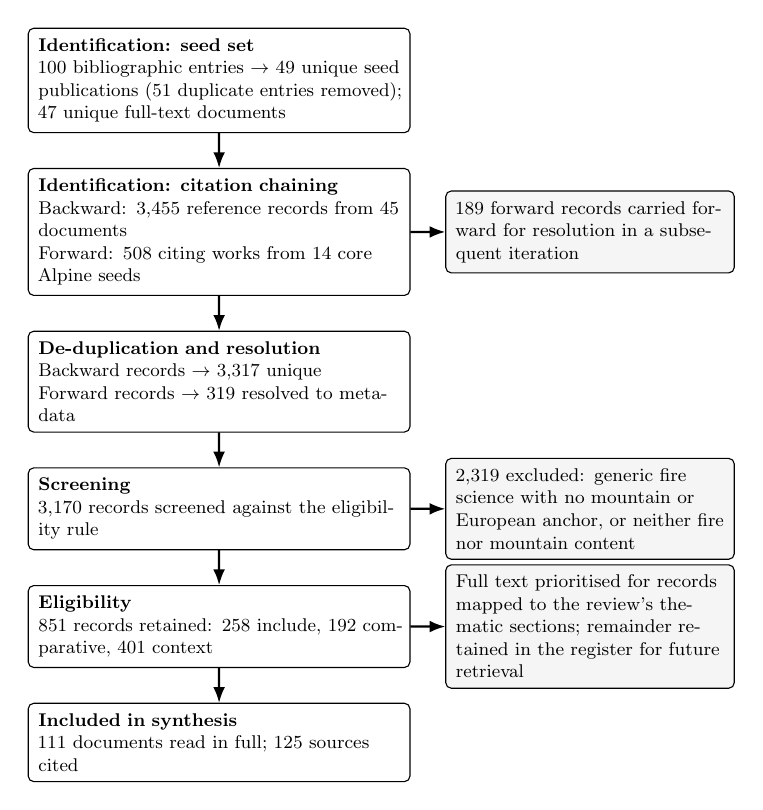
\begin{tikzpicture}[
  scale=0.74, transform shape,
  font=\small,
  box/.style={draw, rounded corners=2pt, align=left, text width=6.2cm, inner sep=5pt},
  side/.style={draw, rounded corners=2pt, align=left, text width=4.6cm, inner sep=5pt, fill=black!4},
  arr/.style={-{Latex[length=2mm]}, thick}
]
\node[box] (seed) {\textbf{Identification: seed set}\\ 100 bibliographic entries $\rightarrow$ 49 unique seed publications (51 duplicate entries removed); 47 unique full-text documents};
\node[box, below=6mm of seed] (chain) {\textbf{Identification: citation chaining}\\ Backward: 3{,}455 reference records from 45 documents\\ Forward: 508 citing works from 14 core Alpine seeds};
\node[box, below=6mm of chain] (dedup) {\textbf{De-duplication and resolution}\\ Backward records $\rightarrow$ 3{,}317 unique\\ Forward records $\rightarrow$ 319 resolved to metadata};
\node[box, below=6mm of dedup] (screen) {\textbf{Screening}\\ 3{,}170 records screened against the eligibility rule};
\node[box, below=6mm of screen] (retain) {\textbf{Eligibility}\\ 851 records retained: 258 include, 192 comparative, 401 context};
\node[box, below=6mm of retain] (incl) {\textbf{Included in synthesis}\\ 111 documents read in full; 125 sources cited};

\node[side, right=6mm of chain] (unres) {189 forward records carried forward for resolution in a subsequent iteration};
\node[side, right=6mm of screen] (excl) {2{,}319 excluded: generic fire science with no mountain or European anchor, or neither fire nor mountain content};
\node[side, right=6mm of retain] (nofull) {Full text prioritised for records mapped to the review's thematic sections; remainder retained in the register for future retrieval};

\draw[arr] (seed) -- (chain);
\draw[arr] (chain) -- (dedup);
\draw[arr] (dedup) -- (screen);
\draw[arr] (screen) -- (retain);
\draw[arr] (retain) -- (incl);
\draw[arr] (chain.east) -- (unres.west);
\draw[arr] (screen.east) -- (excl.west);
\draw[arr] (retain.east) -- (nofull.west);
\end{tikzpicture}
\caption{Flow of records through identification, de-duplication, screening and inclusion. Counts are reported as observed, following the reporting structure of the PRISMA 2020 flow diagram (Table~\ref{tab:prisma}).}
\label{fig:flow}
\end{figure}

\subsection{Screening, coding and evidence capture}

Each record was assigned a tier, a decision and a reason, and each retained record was mapped to one or more sections of this review. For every source cited in the text, a structured evidence note recording study region, method, quantitative results and stated limitations was captured and archived alongside the screening register. Both are provided as supplementary material.

\subsection{Scope of the search and its consequences}

Three properties of the method determine what the corpus contains. Citation chaining reproduces the coverage of its seed set, so topics well represented among the seeds are recovered densely and topics absent from them are recovered weakly. Forward chaining operates on open citation infrastructure, which indexes journal literature comprehensively and national technical reporting and non-English publication sparsely, a material consideration for a range whose fire statistics were harmonised only recently \citep{valese_wildfires_2011, muller_forest_2020}. The expansion phase was confined to material whose full text could be retrieved and archived, which weights the added corpus towards open-access and recent publication.

A subsequent iteration should therefore add database searching with recorded strings and dates, and should target the national fire and forest reporting of the Alpine Convention countries directly, where much of the operational and grey-literature knowledge base resides.


\section{Glossary of Terms}

\begin{description}
    \item[Fire danger] The meteorological and fuel-condition potential for ignition and spread, expressed by an index; a statement about conditions, not about realised fire.
    \item[Fire regime] The realised distribution of fire frequency, size, severity, seasonality and cause over a region and period.
    \item[Burn severity] The degree of fire-induced change to vegetation and soil, commonly estimated remotely; see Section~\ref{sec:cascade} for the limits of this proxy.
    \item[Fuel connectivity] The extent and spatial aggregation of contiguous burnable vegetation, distinct from fuel load.
    \item[Protection forest] Forest whose primary managed function is mitigation of gravitational natural hazards affecting assets below.
    \item[Geohydrological process] Collective term used in the Alpine literature for erosion, rockfall, slides and debris flows driven by the interaction of water and slope material.
    \item[Cascade] A sequence in which one hazard alters the susceptibility of a system to a subsequent, distinct hazard.
    \item[Firebreak] A linear strip from which fuel is removed entirely, intended to stop fire spread.
    \item[Fuel break (\emph{coupure de combustible})] A linear strip in which fuel load and vertical continuity are reduced but the stand is retained; functions primarily as a platform for ground suppression rather than as a barrier.
    \item[Exposure] The elements (people, buildings, infrastructure, habitats, protective forest, livestock and pasture) located where a hazard and its consequences can reach them.
    \item[Vulnerability] The susceptibility of an exposed element to loss given a hazard of stated intensity; distinct from exposure and from hazard, and measured by damage-calibrated or judgement-weighted indicators.
    \item[Ecological vulnerability] Potential loss of ecological value integrated over the post-fire recovery period, combining the value of what burns, the resistance of the vegetation to fire and the time taken to return to pre-fire condition.
\end{description}


% =======================================================
% Bibliography
% =======================================================
\bibliographystyle{apalike}
\bibliography{FireScape_master_v6}

\end{document}
